\chap{序論}

この章では、本修士論文が研究対象とする極低温フェルミ原子気体について概説する。この希薄原子気体では、フェッシュバッハ共鳴と呼ばれる機構を用いることで $\Lisix$ や $\Kafor$ フェルミ原子間にはたらく引力相互作用を自在に制御することができ、単なるフェルミ超流動だけでなく、金属超伝導で議論されている弱結合 BCS(Bardeen-Cooper-Schrieffer)状態から、強い引力相互作用により形成された分子ボソンの BEC(Bose-Einstein condensation)へと連続的に移行する BCS-BEC クロスオーバーが実現している。この系はこれまで、金属超伝導と異なり不純物や欠陥を全く含まないため、様々な相互作用強度における超流動物性を統一的に研究できる系として注目を集めてきたが、近年、遂に系の制御性の高さを活かし、意図的に不純物や乱れを印可することで、不純物効果の系統的な研究も可能となってきている。ここではそうした最近の発展についても説明する。そのうえで、本研究の目的について述べる。

本論文では、簡単のため $\hbar=k_{\text{B}}=1$、体積 $V=1$ とする。
 
\s{極低温フェルミ原子気体}

極低温フェルミ原子気体は、原子間にはたらく相互作用強度をはじめ、密度など様々な物質パラメータに対して高い操作性を有する量子気体である \cite{giorgini2008,bloch2008,ketterle2008}。なかでも超流動研究に対しては、アルカリ金属原子である $\Kafor$ や $\Lisix$ を高温原子源で気化したものが用いられる。気化した原子は、原子線として取り出され、レーザー冷却により数 $\mathrm{mK}$ 程度まで冷やされながら、磁気的、および光学的手法で形成されたトラップポテンシャルに捕獲される \cite{ketterle2008}。さらに蒸発冷却と呼ばれる、高い運動量を持つ原子を選択的に排除し再度熱平衡状態に緩和させる手法により、$10^2\ \mathrm{nK}$ 程度まで冷却される。これらの過程を経て $10^5 \sim 10^7$ 個程度の原子からなる量子縮退したフェルミ原子気体が実現する。


$\Lisix$、および $\Kafor$ のフェルミ原子気体の最大の特徴の 1 つは、フェッシュバッハ共鳴と呼ばれる現象を利用することにより、原子間にはたらく引力相互作用の強度を実験的に自在に制御できる、という点である。フェッシュバッハ共鳴による原子間相互作用制御のために、異なる 2 種類の超微細構造状態にある原子からなる気体が用いられる。具体的には、核スピン $I$ と電子スピン $S$ を合わせた全スピン $F$ について、核スピン $I=1$ の ${}^{6}\mathrm{Li}$ であれば、$\ket{F=1/2, F_z=1/2}$ と $
\ket{F=1/2, F_z=-1/2}$ の 2 状態が、核スピン $I=4$ の ${}^{40}\mathrm{K}$ であれば $\ket{F=9/2, F_z=-9/2}$ と $\ket{F=9/2, F_z=-7/2}$ の 2 状態がよく用いられる \cite{chin2010}。それぞれ全スピン $F$ の $z$ 成分 $F_z$ が異なる 2 つの超微細構造を用いているが、当該研究領域では、これらを電子のスピンになぞらえ、擬スピンアップ($\uar$)、ダウン($\dar$)として表現されることがある。本論文でも、以下ではこれにならい、この 2 種類の超微細構造状態を指すものとして、擬スピンという用語を用いる。

\begin{figure}[t]
\centering
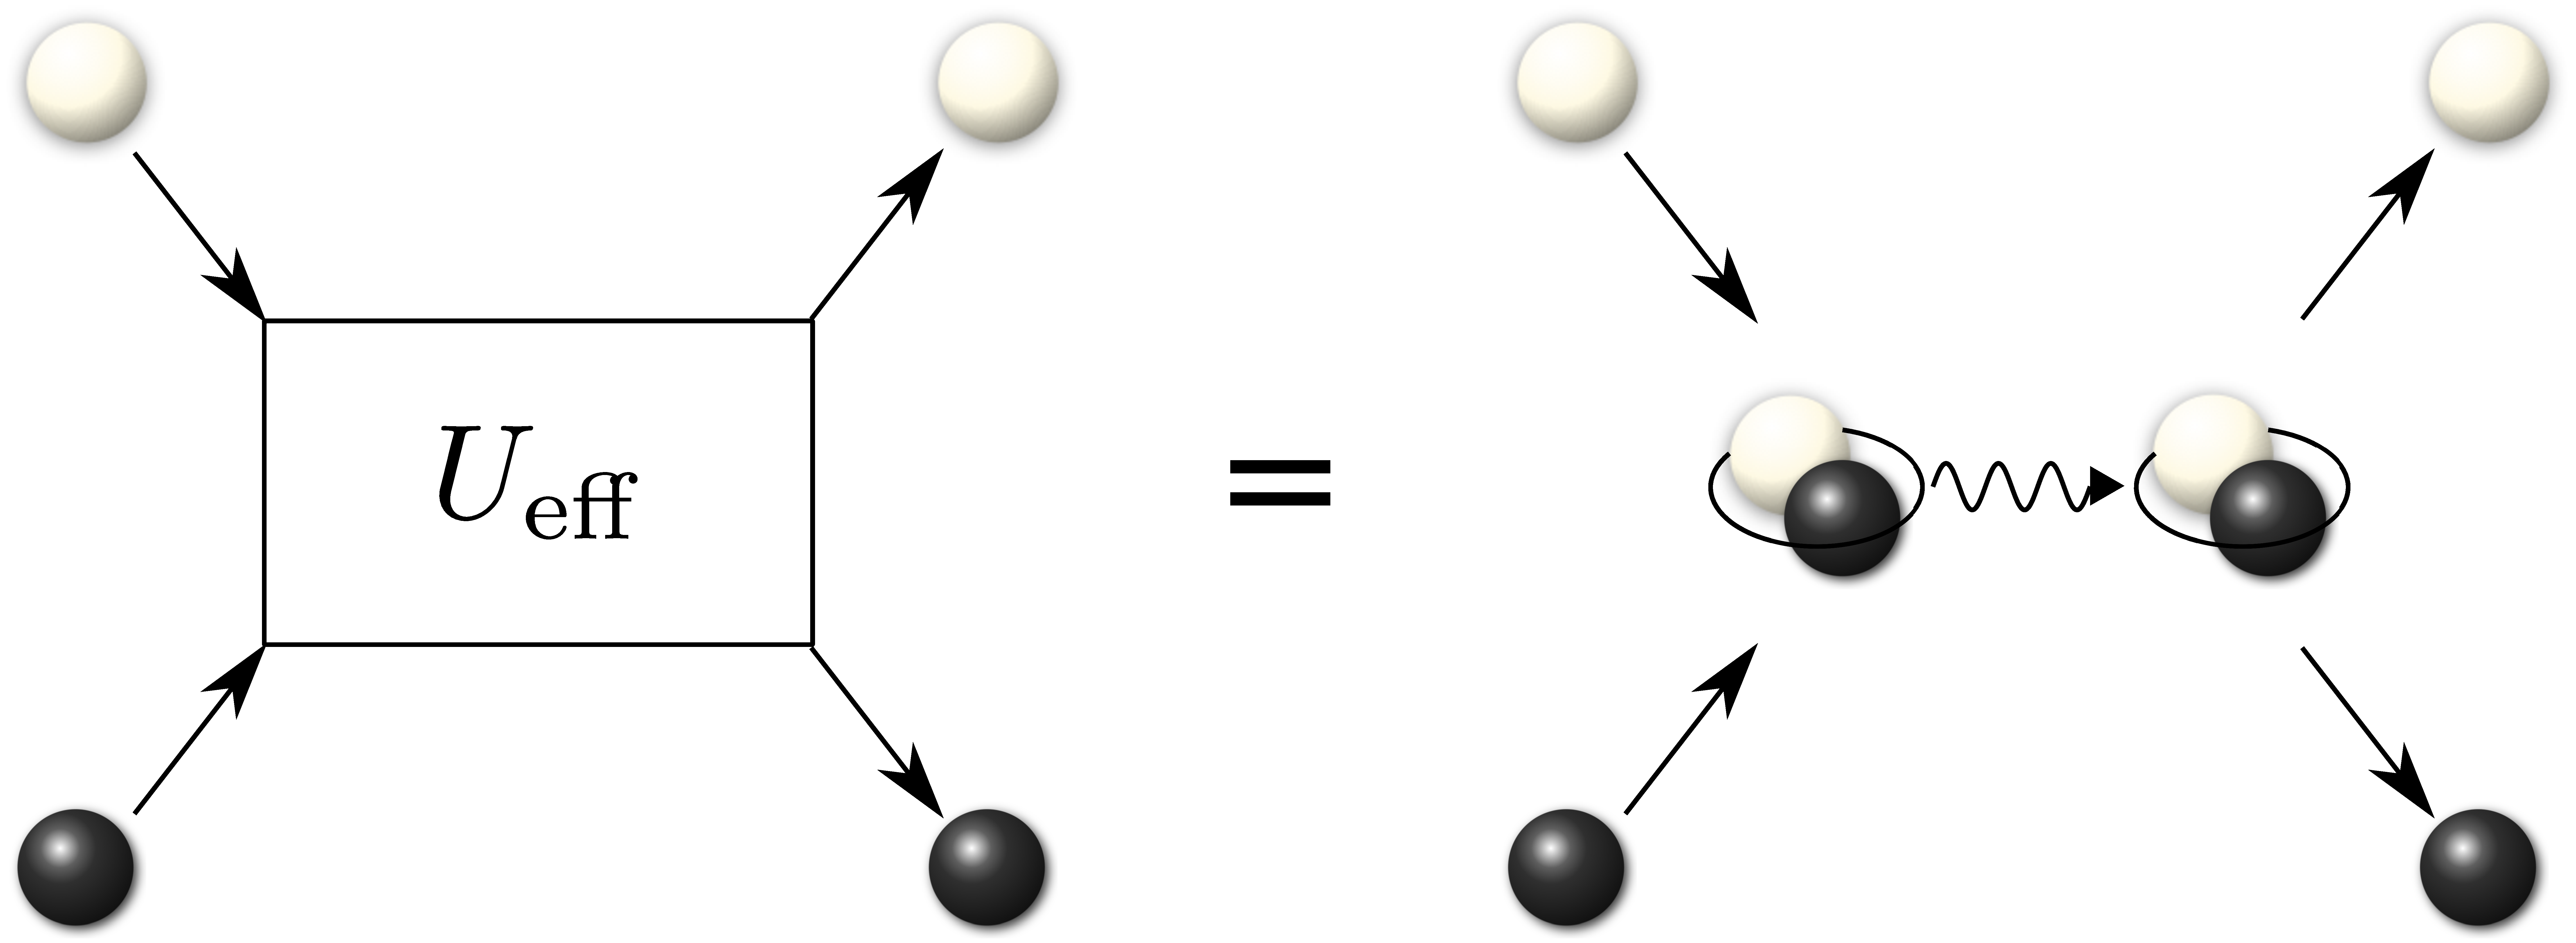
\includegraphics[width=110mm]{eps/feshbach-reso.eps}
\caption{フェッシュバッハ共鳴による原子間相互作用 $U_{\text{eff}}$ の模式図。黒丸と白丸は異なる超微細構造状態のフェルミ原子を表す。フェッシュバッハ共鳴では、この 2 つの原子が散乱される際、中間状態としてフェッシュバッハ分子の形成(図中波線部分)と、解離がおこる。この分子状態(共鳴束縛状態)のエネルギーをゼーマン効果を利用し、外部磁場で制御することで 2 つのフェルミ原子(白丸、黒丸)間の相互作用強度を変えることができる。式 (\ref{eq:intro:ueff}) にはこれ以外の相互作用 $U$ も加えてある。
}
\label{fig:feshbach}
\end{figure}

フェッシュバッハ共鳴とは、擬スピン $\uar$, $\dar$ の 2 つのフェルミ原子(open channel)の全運動エネルギーと、この~2~原子が束縛分子状態(closed channel)を形成した際のエネルギーが一致する場合に、図 \ref{fig:feshbach} に模式的に示したように共鳴散乱が起こる現象である \cite{feshbach1962}。この共鳴束縛状態にあるフェルミ原子は、“解離”状態にあるフェルミ原子とは異なる超微細構造状態であるため、open channel と closed channel では外部磁場によるゼーマン効果が異なる。このため系に印可する磁場により、共鳴束縛状態(フェッシュバッハ分子)と open channel にある 2 原子とのエネルギー差を制御することができる。今、共鳴束縛状態と open channel にある 2 つのフェルミ原子のエネルギー差を $2 \nu$、open channel から closed channel への遷移振幅を $g$、フェッシュバッハ共鳴とは関係ない原因による擬スピン $\uar$ と $\dar$ 間の相互作用を $U$ とすると、$g$ について 2 次摂動の範囲で擬スピン $\uar$、$\dar$ の 2 状態にあるフェルミ原子間の有効相互作用として次式を得る \cite{ohashi2005}。
\beq
U_{\text{eff}} = U - \frac{g^2}{2\nu}.\label{eq:intro:ueff}
\eeq
$2\nu=0$ となるフェッシュバッハ共鳴磁場を $B_0$ とすれば、共鳴点付近では定数 $\alpha$ を用い $2 \nu = \alpha (B-B_0)$ と表せる。このように有効相互作用が外部磁場 $B$ の値に依存して変化する時、2 つのフェルミ原子($\uar$、$\dar$)間の散乱長や散乱断面積などの物理量も同時に変化する。特に、$s$ 波散乱長 $a_s$ は、
\begin{figure}[t]
\centering
%\vspace{24mm}
%C. A. Regal, and D. S. Jin, Phys. Rev. Lett. 90, 230404 (2003).\\
%Figure 3.
%\vspace{24mm}
%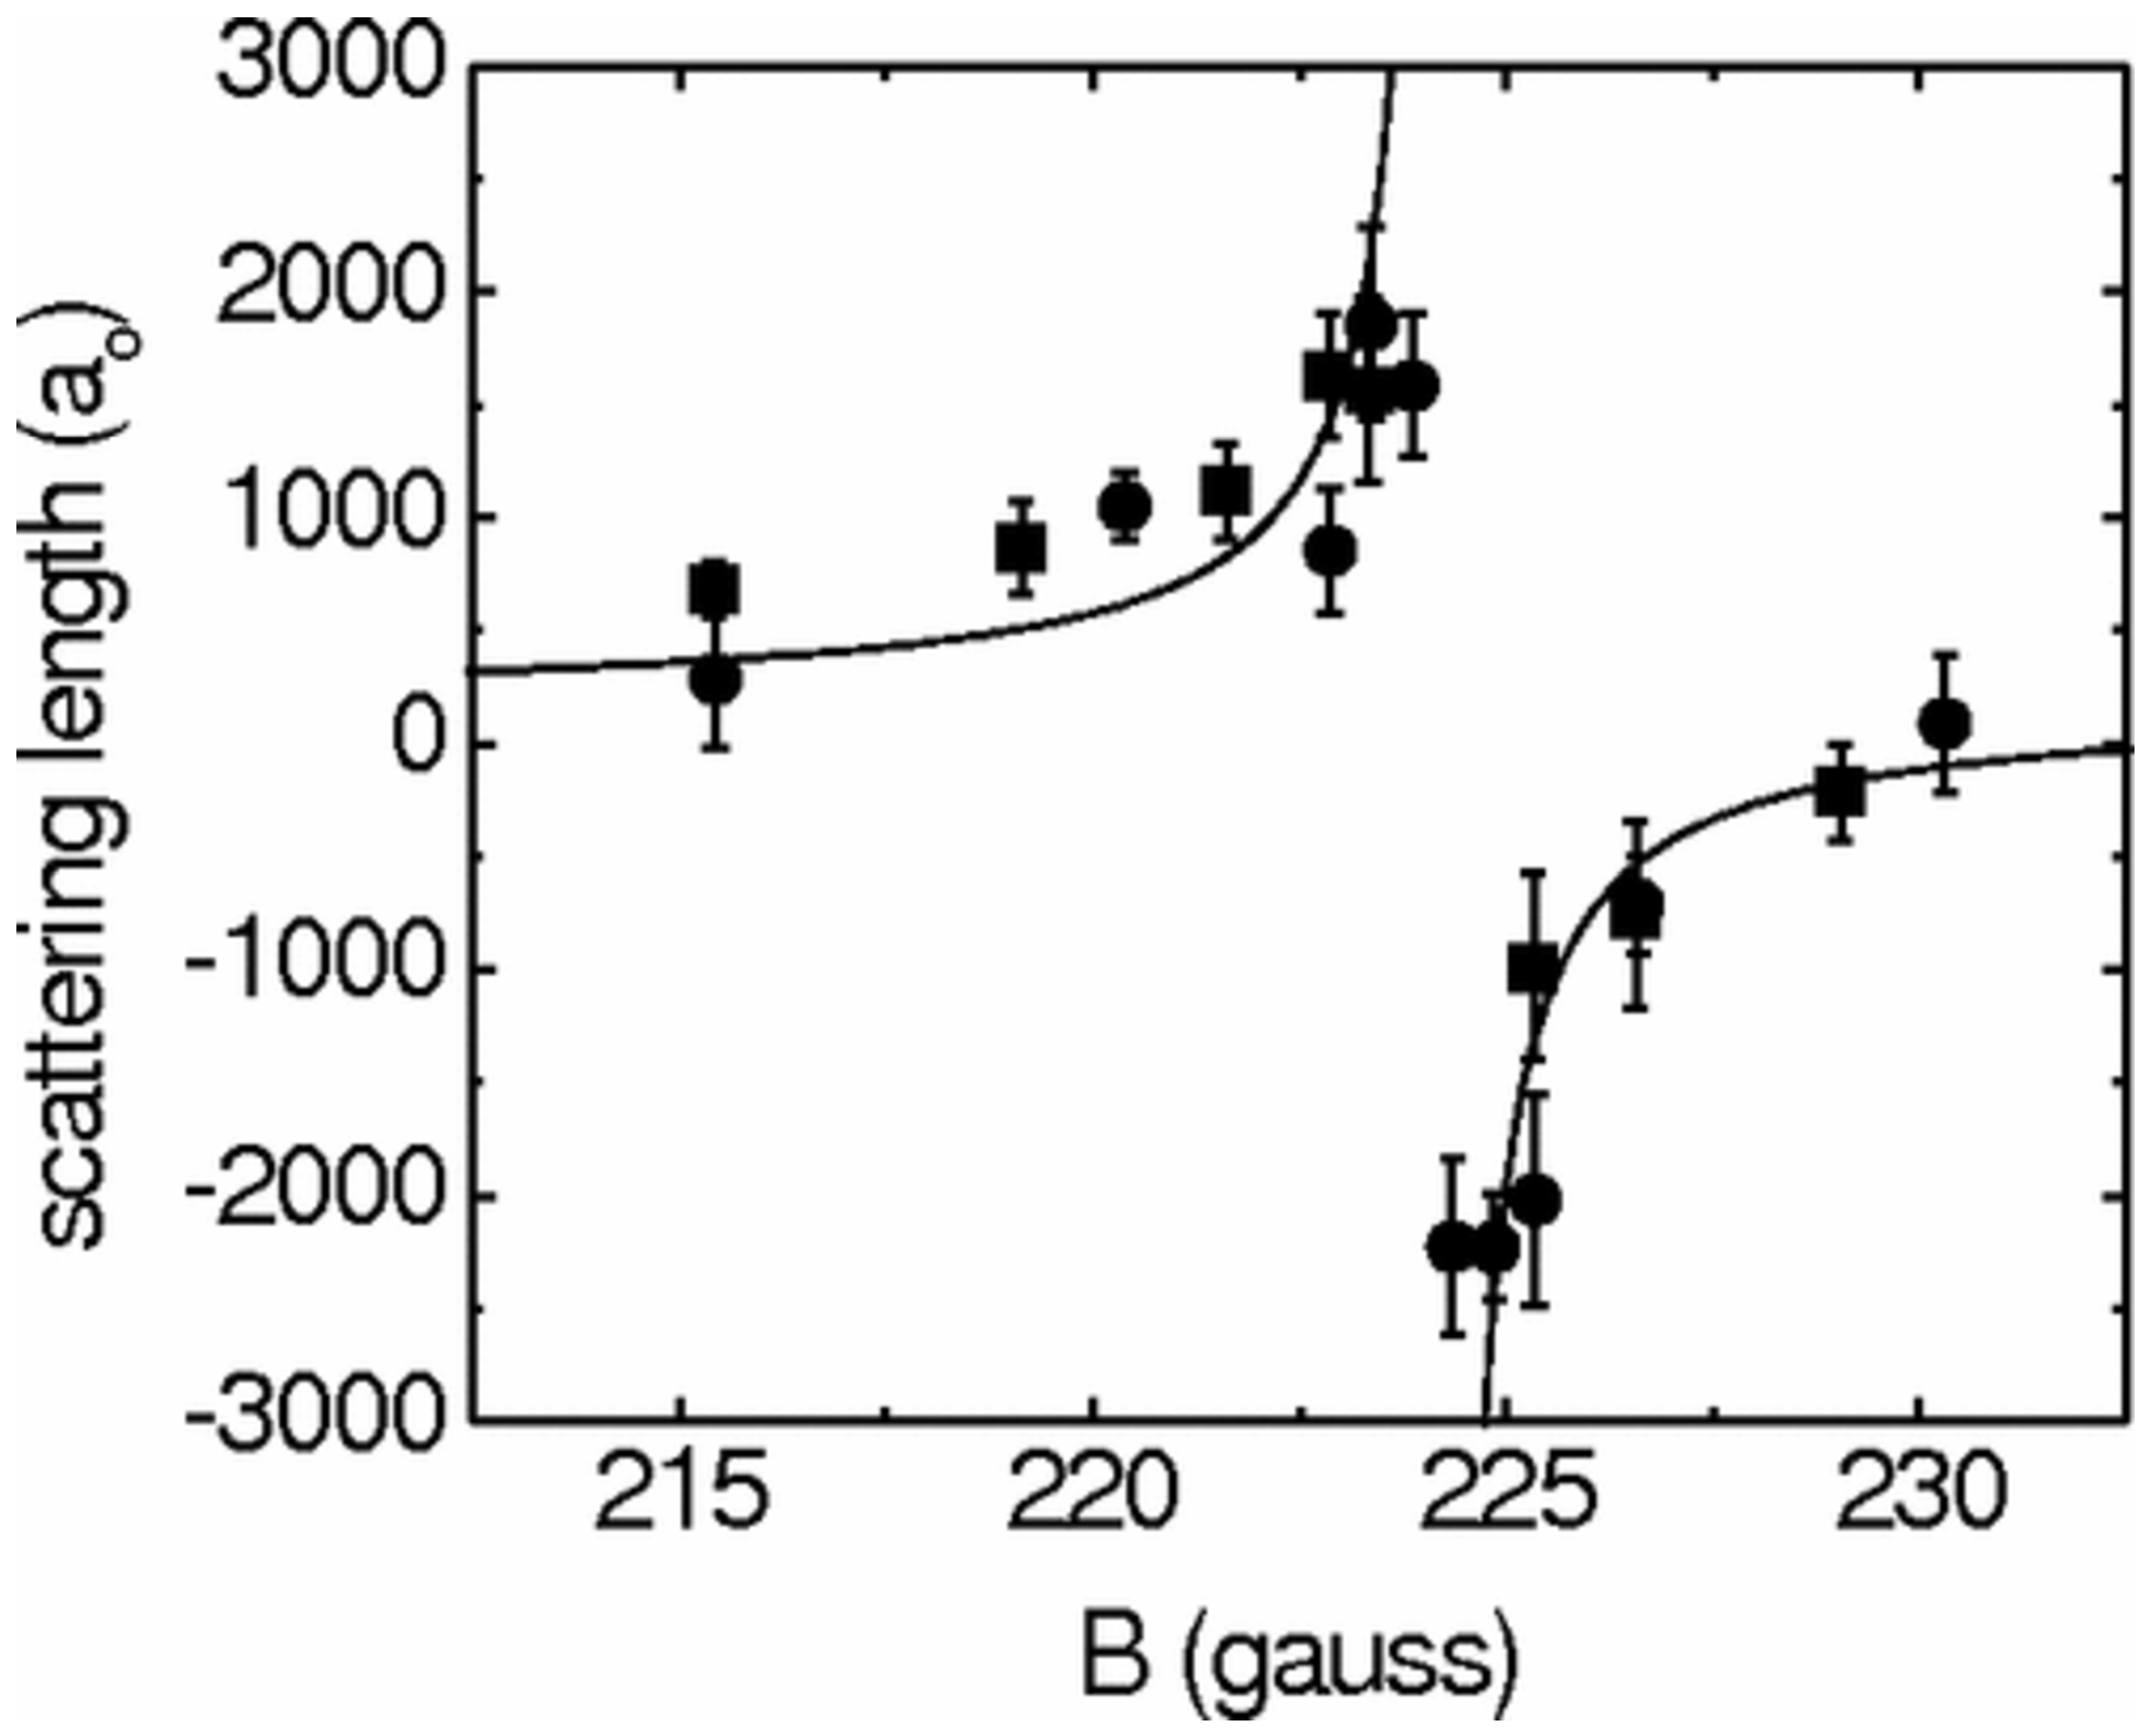
\includegraphics[width=70mm,height=56mm]{eps/medium.eps}
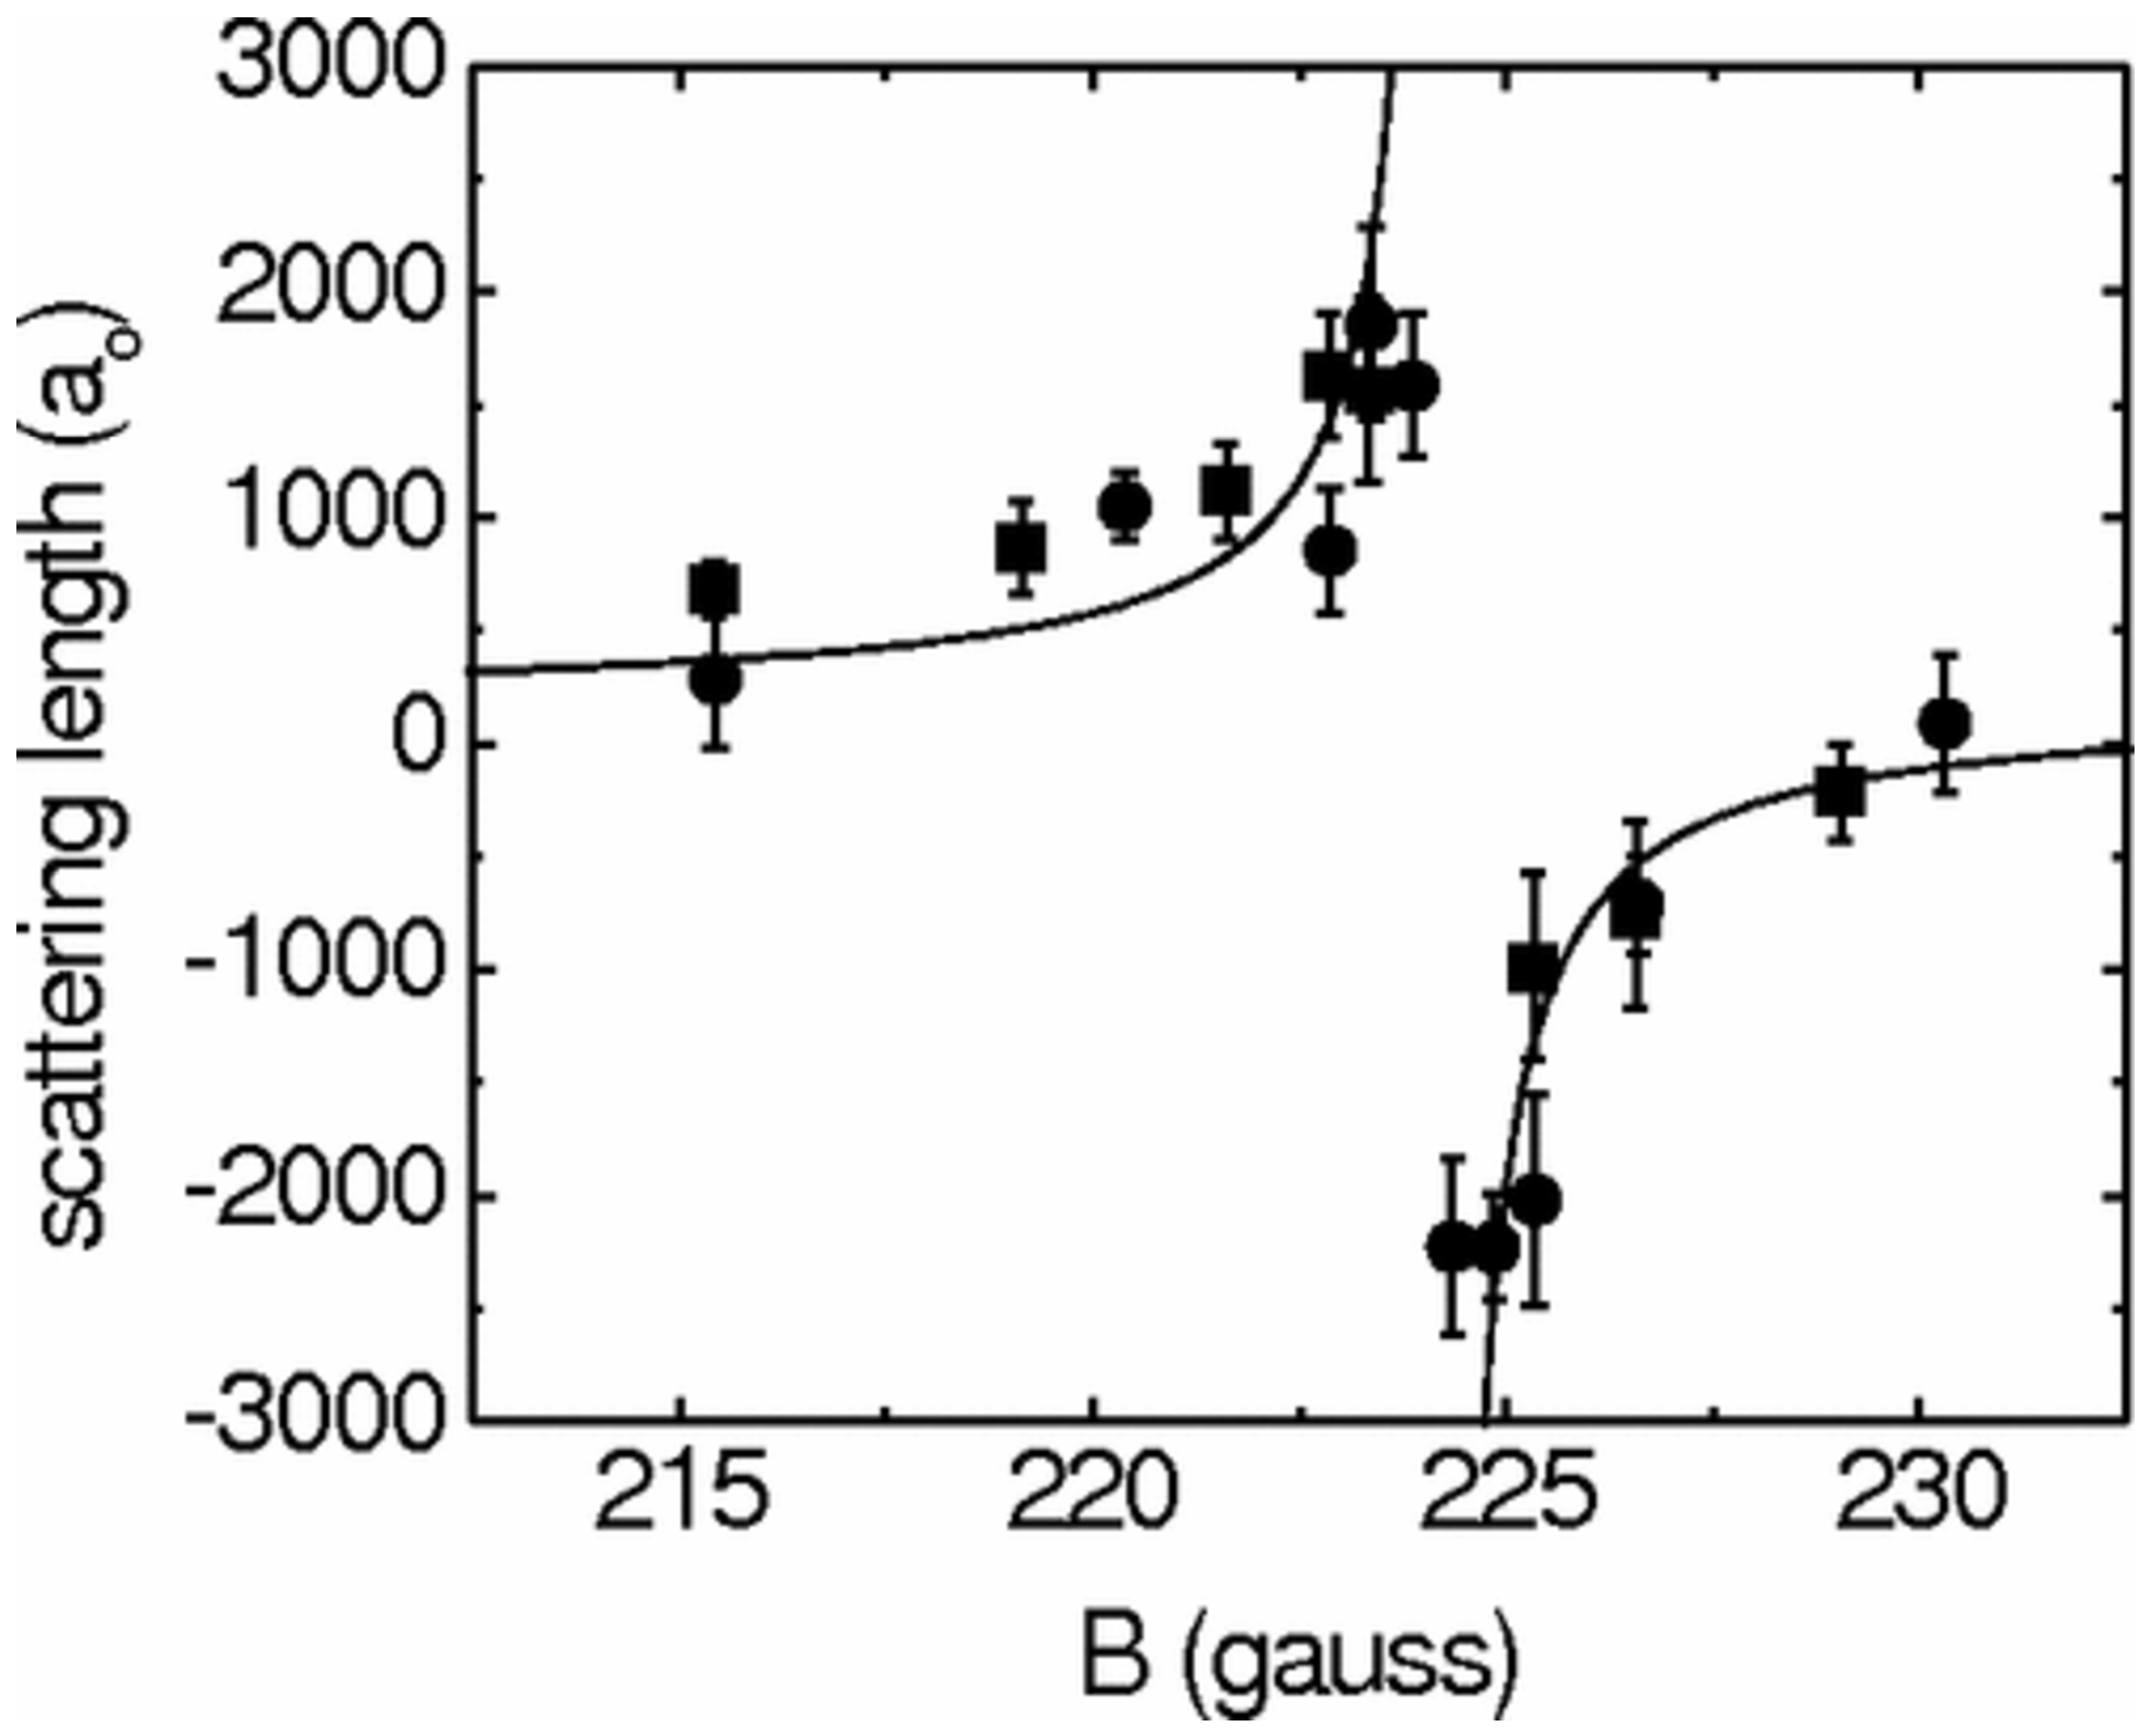
\includegraphics[width=70mm]{eps/medium.eps}
\caption{極低温 $\Kafor$ フェルミ気体で観測された、超微細構造状態 $\ket{F=9/2,F_z=-9/2}$ と $\ket{F=9/2, F_z=-7/2}$ にある原子間のフェッシュバッハ共鳴磁場付近の散乱長の磁場依存性\cite{regal2003}。$a_0$ はボーア半径。実線は、実験結果をフィッティングしたもの。共鳴磁場は $B_0=224.21\pm0.05\  \text{G}$。}
\label{fig:sscatter}
\end{figure}
\beq
a_s (B) = a_s^{\text{bg}}\left(1-\frac{\delta B}{B-B_0}\right),\label{eq:intro:askfi}
\eeq
とかける \cite{pethick2008}。ここで $a_s^{\text{bs}}$ はフェッシュバッハ共鳴磁場 $B_0$ から十分離れた磁場での散乱長の値を表し、$\delta B$ と共に実験的に決めることができる。この$s$ 波散乱長の磁場依存性は、相互作用による準位のエネルギーシフトを測定することで図 \ref{fig:sscatter} のように観測されており、式 (\ref{eq:intro:askfi}) から予想される通り、共鳴磁場 $B_0=224.21\pm0.05\  \text{G}$ を境に散乱長の符号が反転している。$s$ 波散乱長は散乱断面積を通しても観測されている \cite{loftus2002}。

\begin{figure}[t]
\centering
%\vspace{28mm}
%C. A. Regal, M. Greiner, and D. S. Jin, Phys. Rev. Lett. 92, 040403 (2004).\\
%Figure 4.
%\vspace{28mm}
%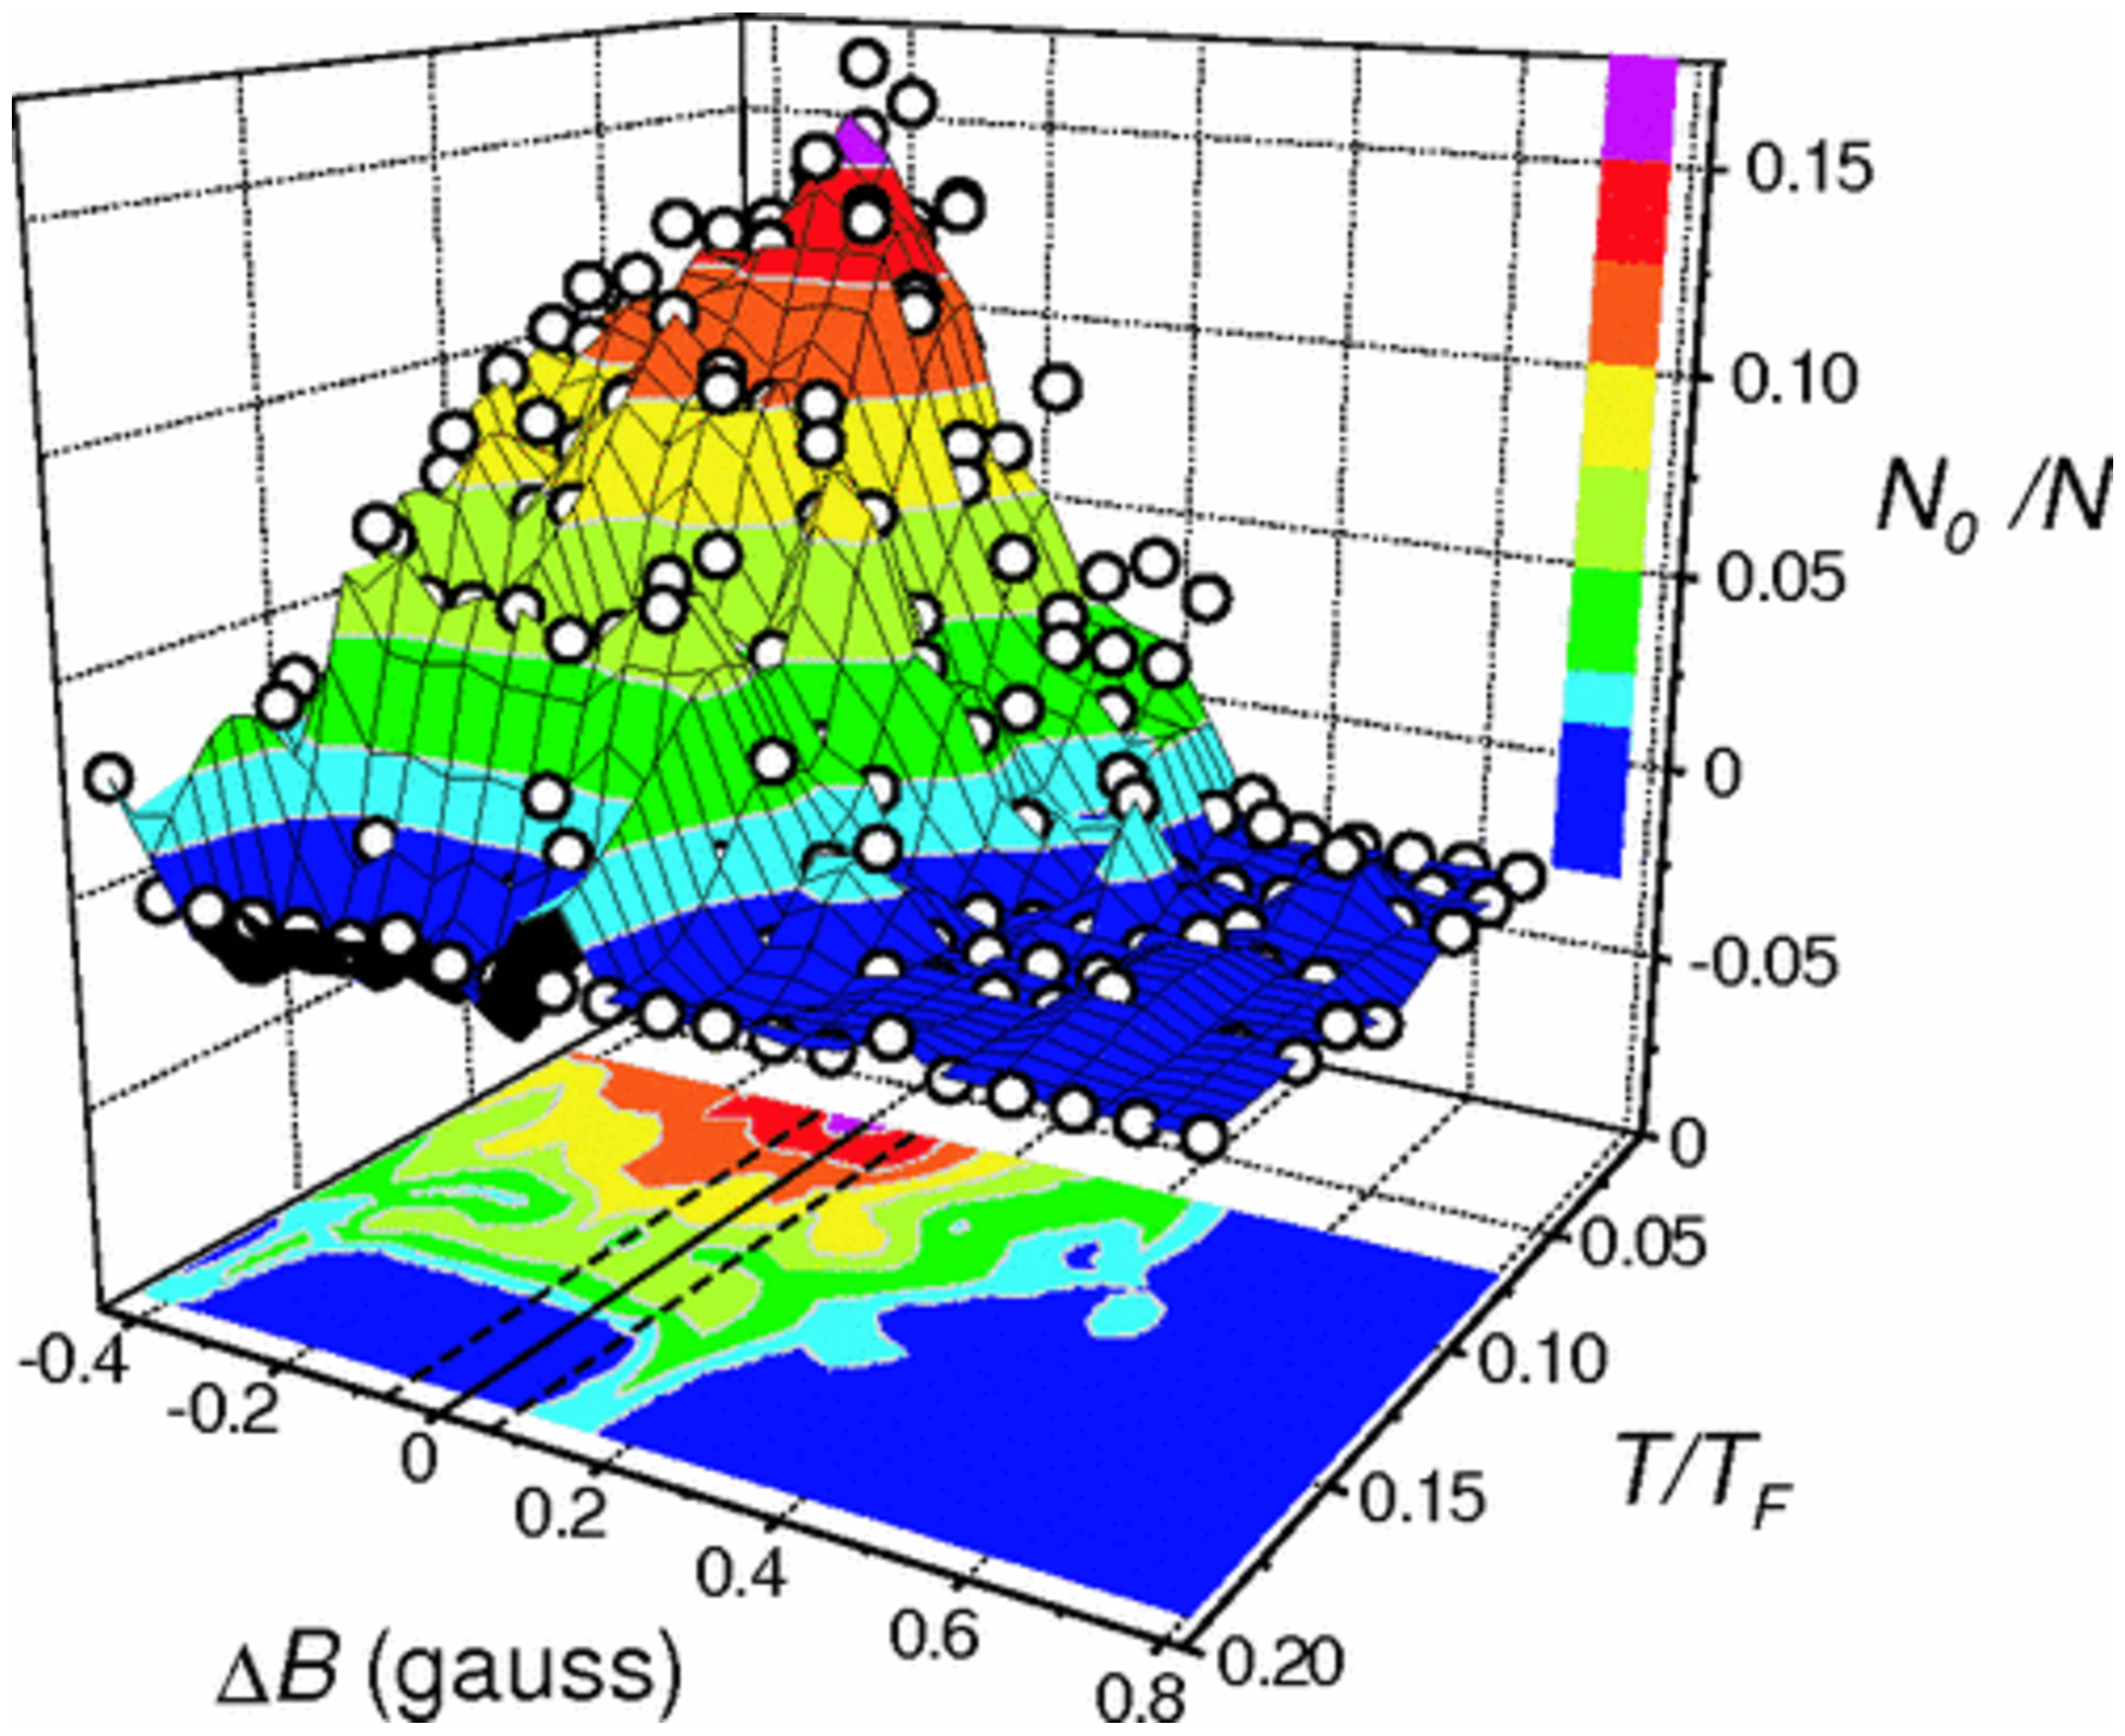
\includegraphics[width=80mm,height=60mm]{eps/bcs-bec-pota.eps}
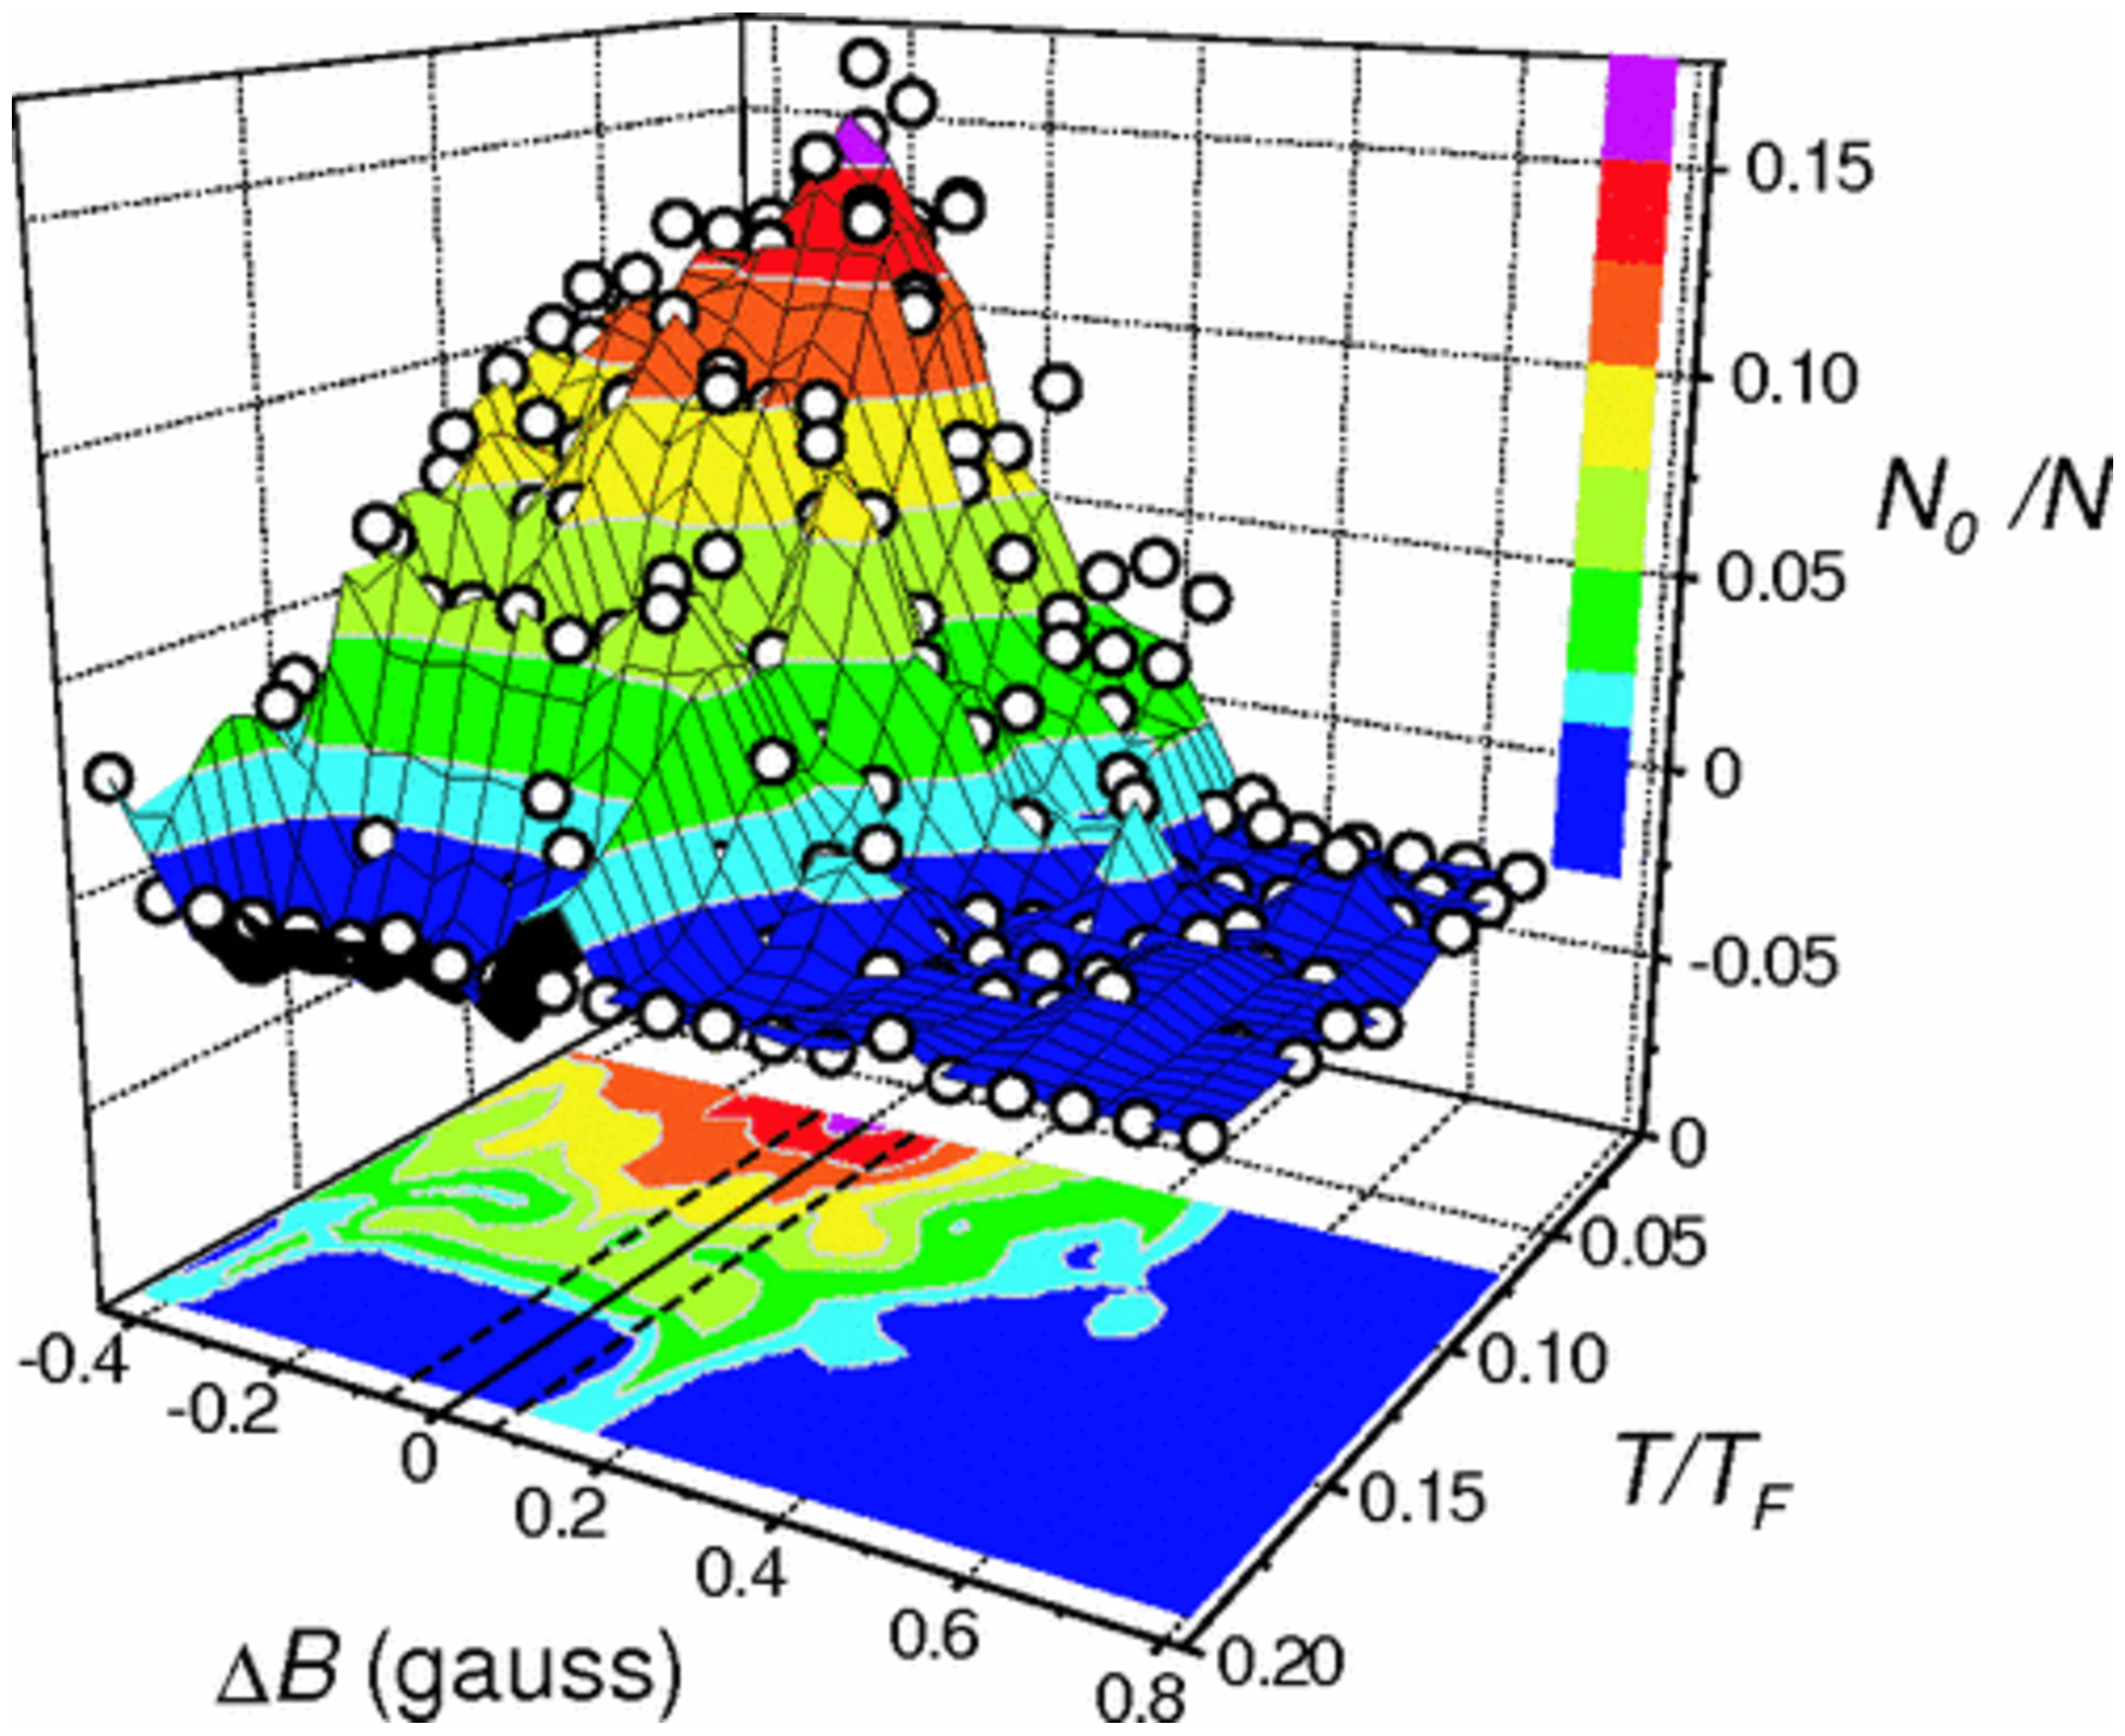
\includegraphics[width=80mm]{eps/bcs-bec-pota.eps}
\caption{${}^{40}\mathrm{K}$ フェルミ原子気体で観測された超流動転移と BCS-BEC クロスオーバー\cite{regal2004}。原子気体は $\ket{F, F_z} = \ket{9/2,-9/2}, \ket{9/2, -7/2}$ で構成される。図は凝縮粒子数(重心運動量 0 にボース・アインシュタイン凝縮しているクーパー対の数) $N_0$ の相互作用、温度依存性を示しており、この実験では $N_0/N>0$ の領域を超流動状態と判定している。図中の $\Delta B$ は、フェッシュバッハ共鳴磁場からのずれであり、この軸は原子間相互作用の強さを表す。$\Delta B>0$ は弱結合、$\Delta B<0$ は強結合の領域に対応している。$N_0/N$ が有限となり始めるのはこの図では大体水色のあたりであり、底面の水色部分が超流動転移温度 $\tc$ と考えられる。$\Delta B$ が下がる(=引力相互作用が強くなる)につれ、$\tc$ は上昇する。$\Delta B <0$ の強結合側では一定値 $T/\tc \sim 0.17$ をとる。このふるまいは図 \ref{fig:bcsbecsouzu} に示す相図中の $\tc$ のふるまいと定性的に一致している。}
\label{fig:bcsbecpota}
\end{figure}


上述のフェッシュバッハ共鳴による可変な引力相互作用強度を利用することで、フェルミ超流動の性質を、弱結合 BCS 理論で記述されるものから、強い引力相互作用で形成された分子ボソンの BEC で記述される状態へと相転移なく連続的に変化させることができる(BCS-BEC クロスオーバー)。図 \ref{fig:bcsbecpota} は $\Kafor$ フェルミ原子ガスにおいて、凝縮粒子数(ボース・アインシュタイン凝縮しているクーパー対の数)を測定することで、BCS-BEC クロスオーバーを観測した実験結果である \cite{regal2004}。

図 \ref{fig:bcsbecsouzu} は、BCS-BEC クロスオーバー領域におけるフェルミ原子気体の温度-相互作用相図の模式図である。擬スピンの異なるフェルミ原子間の引力相互作用が弱い、$\askfi\ltsim -1$ の領域(弱結合領域、または BCS 領域)では、低温での金属超伝導で議論されている BCS 状態でよく説明される超流動状態に相転移する。一方、引力相互作用が強い、$\askfi \gtsim +1$ の領域(強結合領域、またはBEC 領域)では、超流動転移温度 $\tc$ 以上の常流動状態の時点で強い引力相互作用により 2 体束縛状態である分子ボソンをすでに形成し、低温になると、この分子ボソンが BEC を起こし超流動状態へと相転移する。図 \ref{fig:bcsbecsouzu} に示すように弱結合、強結合側のこれら超流動状態間には相転移はなく、原子間引力相互作用を制御することで一方から他方にクロスオーバーする \cite{eagles1969,leggett1980,sademelo1993}。

相図 \ref{fig:bcsbecsouzu} において、2 体の散乱長 $\as$ が発散するユニタリ極限 $\askfi=0$ 付近の領域($-1\ltsim \askfi \ltsim 1$)は、ユニタリ領域と呼ばれ、クーパー対形成と解離の頻繁な繰り返しで特徴付けられる超流動ゆらぎが顕著な領域である。この領域では強い超流動ゆらぎにより、擬ギャップと呼ばれる、超流動転移温度以上でも超流動ギャップと類似の構造が 1 粒子状態密度に現れる現象が起こると理論的に指摘されている \cite{gaebler2010,sagi2015}。この擬ギャップ現象はアンダードープ領域の銅酸化物高温超伝導体では実際に実験的にも観測されている \cite{kugler2001}。フェルミ原子気体では 1 粒子状態密度を直接観測する実験結果が現在のところ存在しないため、実験的には完全には確認されていないが、光原子分光スペクトルではその存在を示唆する結果が $\Kafor$ フェルミ原子ガスに対し報告されている \cite{stewart2008}。

\begin{figure}[t]
\centering
\includegraphics[width=90mm]{eps/bcs-bec-cross.eps}
\caption{冷却フェルミ原子気体における BCS-BEC クロスオーバーの相図(模式図)。縦軸が温度 $T$ をフェルミ縮退温度 $T_{\text{F}}$ で規格化したもの、横軸は原子間相互作用を $s$ 波散乱長の逆数でスケールしたもの。$\kf$ はフェルミ波数。$\tc$ の線は原子間相互作用に対する $T$ 行列理論(付録 \ref{sec:append:pure})に基づく。このスケールでは、$\askfi<0$ が弱結合 BCS 側であり、$\askfi>0$ が強結合 BEC 側である。BCS 領域では擬スピン $\uar$ と $\dar$ のフェルミ原子が低温でクーパー対を形成し BCS 状態となる。BEC 領域では $\tc$ 以上の常流動状態ですでに分子ボソンが形成され、分子ボース気体が BEC を起こすことで超流動状態となる。$-1\ltsim \askfi \ltsim 1$ はユニタリ領域と呼ばれ、超流動ゆらぎが強い領域になっており、$\tc$ 以上で形成されたクーパー対により、$\tc$ 以上でも 1 粒子状態密度にギャップ現れる領域(擬ギャップ領域)が相図上に存在する。この相図において相転移は $\tc$ の線上のみで起こり、“フェルミ原子気体”と“擬ギャップ”、および“擬ギャップ”と“分子ボース気体”の境界は、相転移を伴わないクロスオーバーである。また図中黄色の丸は擬スピン $\uar$、$\dar$ のフェルミ原子気体の状況を各領域で模式的に示したものである。}
\label{fig:bcsbecsouzu}
\end{figure}


BCS-BEC クロスオーバーは理論的には、絶対零度($T=0$)では平均場 BCS 理論に基づく BCS-Leggett 理論で理解される。通常の弱結合 BCS 理論では、化学ポテンシャル $\cpt$ はフェルミエネルギー $\epsilon_{\text{F}}$ に等しいとして BCS ギャップ方程式のみを解いて超伝導(超流動)秩序パラメータ $\del$ を求めるのに対し、BCS-Leggett 理論では、$\del$ と $\cpt$ を自己無撞着に決定する。これにより強結合極限において 2 体束縛状態としての分子ボソンの BEC 状態を正しく記述できることが知られている。この BCS-BEC クロスオーバー理論は熱ゆらぎのない絶対零度で正当化されるが、有限温度では超流動ゆらぎの効果を記述できないため使うことができない。有限温度の BCS-BEC クロスオーバーを記述するためには、平均場近似をこえて超流動ゆらぎの効果を取り扱える強結合理論が必要となる \cite{sademelo1993,Nozieres1985,perali2002}。


%以上のようにフェッシュバッハ共鳴による可変な相互作用を利用して、BCS-BEC クロスオーバーが実現されている。


\s{金属超伝導体における不純物効果の研究}

冷却原子気体において、近年不純物効果の実験が実現され\cite{kharamov2012,konishi2016,billy2008,jendrezejewski2012}、理論的にも注目を集めている\cite{han2011,palestini2013,che2016}。本修士論文は冷却フェルミ原子気体の BCS-BEC クロスオーバー領域における非磁性不純物効果を研究するが、ここでは、この分野において先行している、金属超伝導における不純物効果について説明する。

金属超伝導体の熱力学的性質に対する不純物効果は、対破壊パラメータと呼ばれる、不純物による電子の散乱効果における時間反転対称性の破れを表すパラメータによって系統的に理解することができる\cite{abrikosov1961,maki1968}。特に、非磁性不純物のように時間反転対称性を破らない不純物については、アンダーソンの定理が知られている\cite{anderson1959}。この定理は、BCS 理論によって記述される($s$ 波)超伝導状態の熱力学的性質(例えば超伝導転移温度 $\tc$)は非磁性不純物の影響を受けないことを主張する。これはBCS 超伝導状態が互いに時間反転対称な状態にある電子同士によるクーパー対に基づいていることによる性質である。時間反転対称性を守る非磁性不純物は、クーパー対を形成している 2 電子を等しく散乱するため、対を破壊する効果をもたらさず、結果として超伝導の熱力学的性質に影響を与えない。

磁性不純物のように時間反転対称性を破る場合は、クーパー対を構成する 2 電子に対し異なる散乱効果をもたらすために対破壊が生じ、超伝導状態に大きな影響を与える。実際、磁性不純物による超伝導転移温度の減少\cite{abrikosov1961}やギャップレス超伝導\cite{maki1968}、さらには超伝導ギャップ中に局在する励起状態\cite{yazdani1997,shiba1968,shiba1973} の生成等の効果が知られている。

ただし、非磁性不純物のように対破壊を起こさない不純物であっても、超伝導の性質に影響を与える場合がある。超伝導転移温度近傍の常伝導状態では、超流動揺らぎの影響で電気伝導率が増大する現象が知られている\cite{Ferrell1969}。この現象はパラコンダクティビティと呼ばれるが、非磁性不純物が系に存在すると電子の平均自由工程が短くなることで、この効果が増大することが知られている \cite{Ferrell1969}。これは非磁性不純物によって超伝導揺らぎが強くなることに因るものである。

以上概説したように、金属超伝導における不純物効果は詳しく調べられているが、従来型の多くの金属超伝導が格子振動(フォノン)を電子間引力相互作用の起源としていることから、デバイ周波数という物理的なカットオフが存在し、それがフェルミエネルギー $\eqf$ に比べ十分小さいことを暗に仮定している \cite{maki1968}。すなわちフェルミ面近傍の(カットオフエネルギーの範囲内にある)状態以外は超伝導現象には影響せず、それゆえ電子-正孔対称性が満たされた(あるいは暗に仮定された)状態で議論されている。上述のアンダーソンの定理の証明もこの対称性を仮定している。もちろん、通常の金属ではフェルミエネルギー $\eqf$ は $10^{4} \sim 10^{5}\ \mathrm{K}$ のオーダーであるのに対し、デバイ周波数は $\omega_{\text{D}} \simeq 10^{1}\sim 10^{3}\ \mathrm{K}$ であるため、フェルミ面近傍の 1 粒子状態密度のエネルギー依存性が非常に顕著であるような特殊な場合を除し、この仮定は合理的なものである。一方、BCS-BEC クロスオーバーが観測された極低温フェルミ原子気体では、フェッシュバッハ共鳴による引力相互作用を用いているため、フォノンのデバイ周波数のような、物理的なカットオフは存在せず、粒子間相互作用は全エネルギー領域で作用するため、粒子-ホール対称性は成り立たない。そのため、非磁性不純物であっても超流動状態に影響を与える可能性がある。さらに冷却原子系では、超流動ゆらぎにより、ユニタリ領域において $\tc$ 以上の正常相で擬ギャップが現れると期待されているが、金属超伝導におけるパラコンダクティビティと同様に、非磁性不純物により擬ギャップ現象が影響を受ける可能性がある。


\begin{figure}[t]
\centering
%\vspace{22mm}
%A. Y. Khramov, A. H. Hansen, A. O. Jamison, W. H. Dowd, and S. Gupta,\\
% Phys. Rev. A 86, 032705 (2002).\\
%Figure 1.
%\vspace{22mm}
%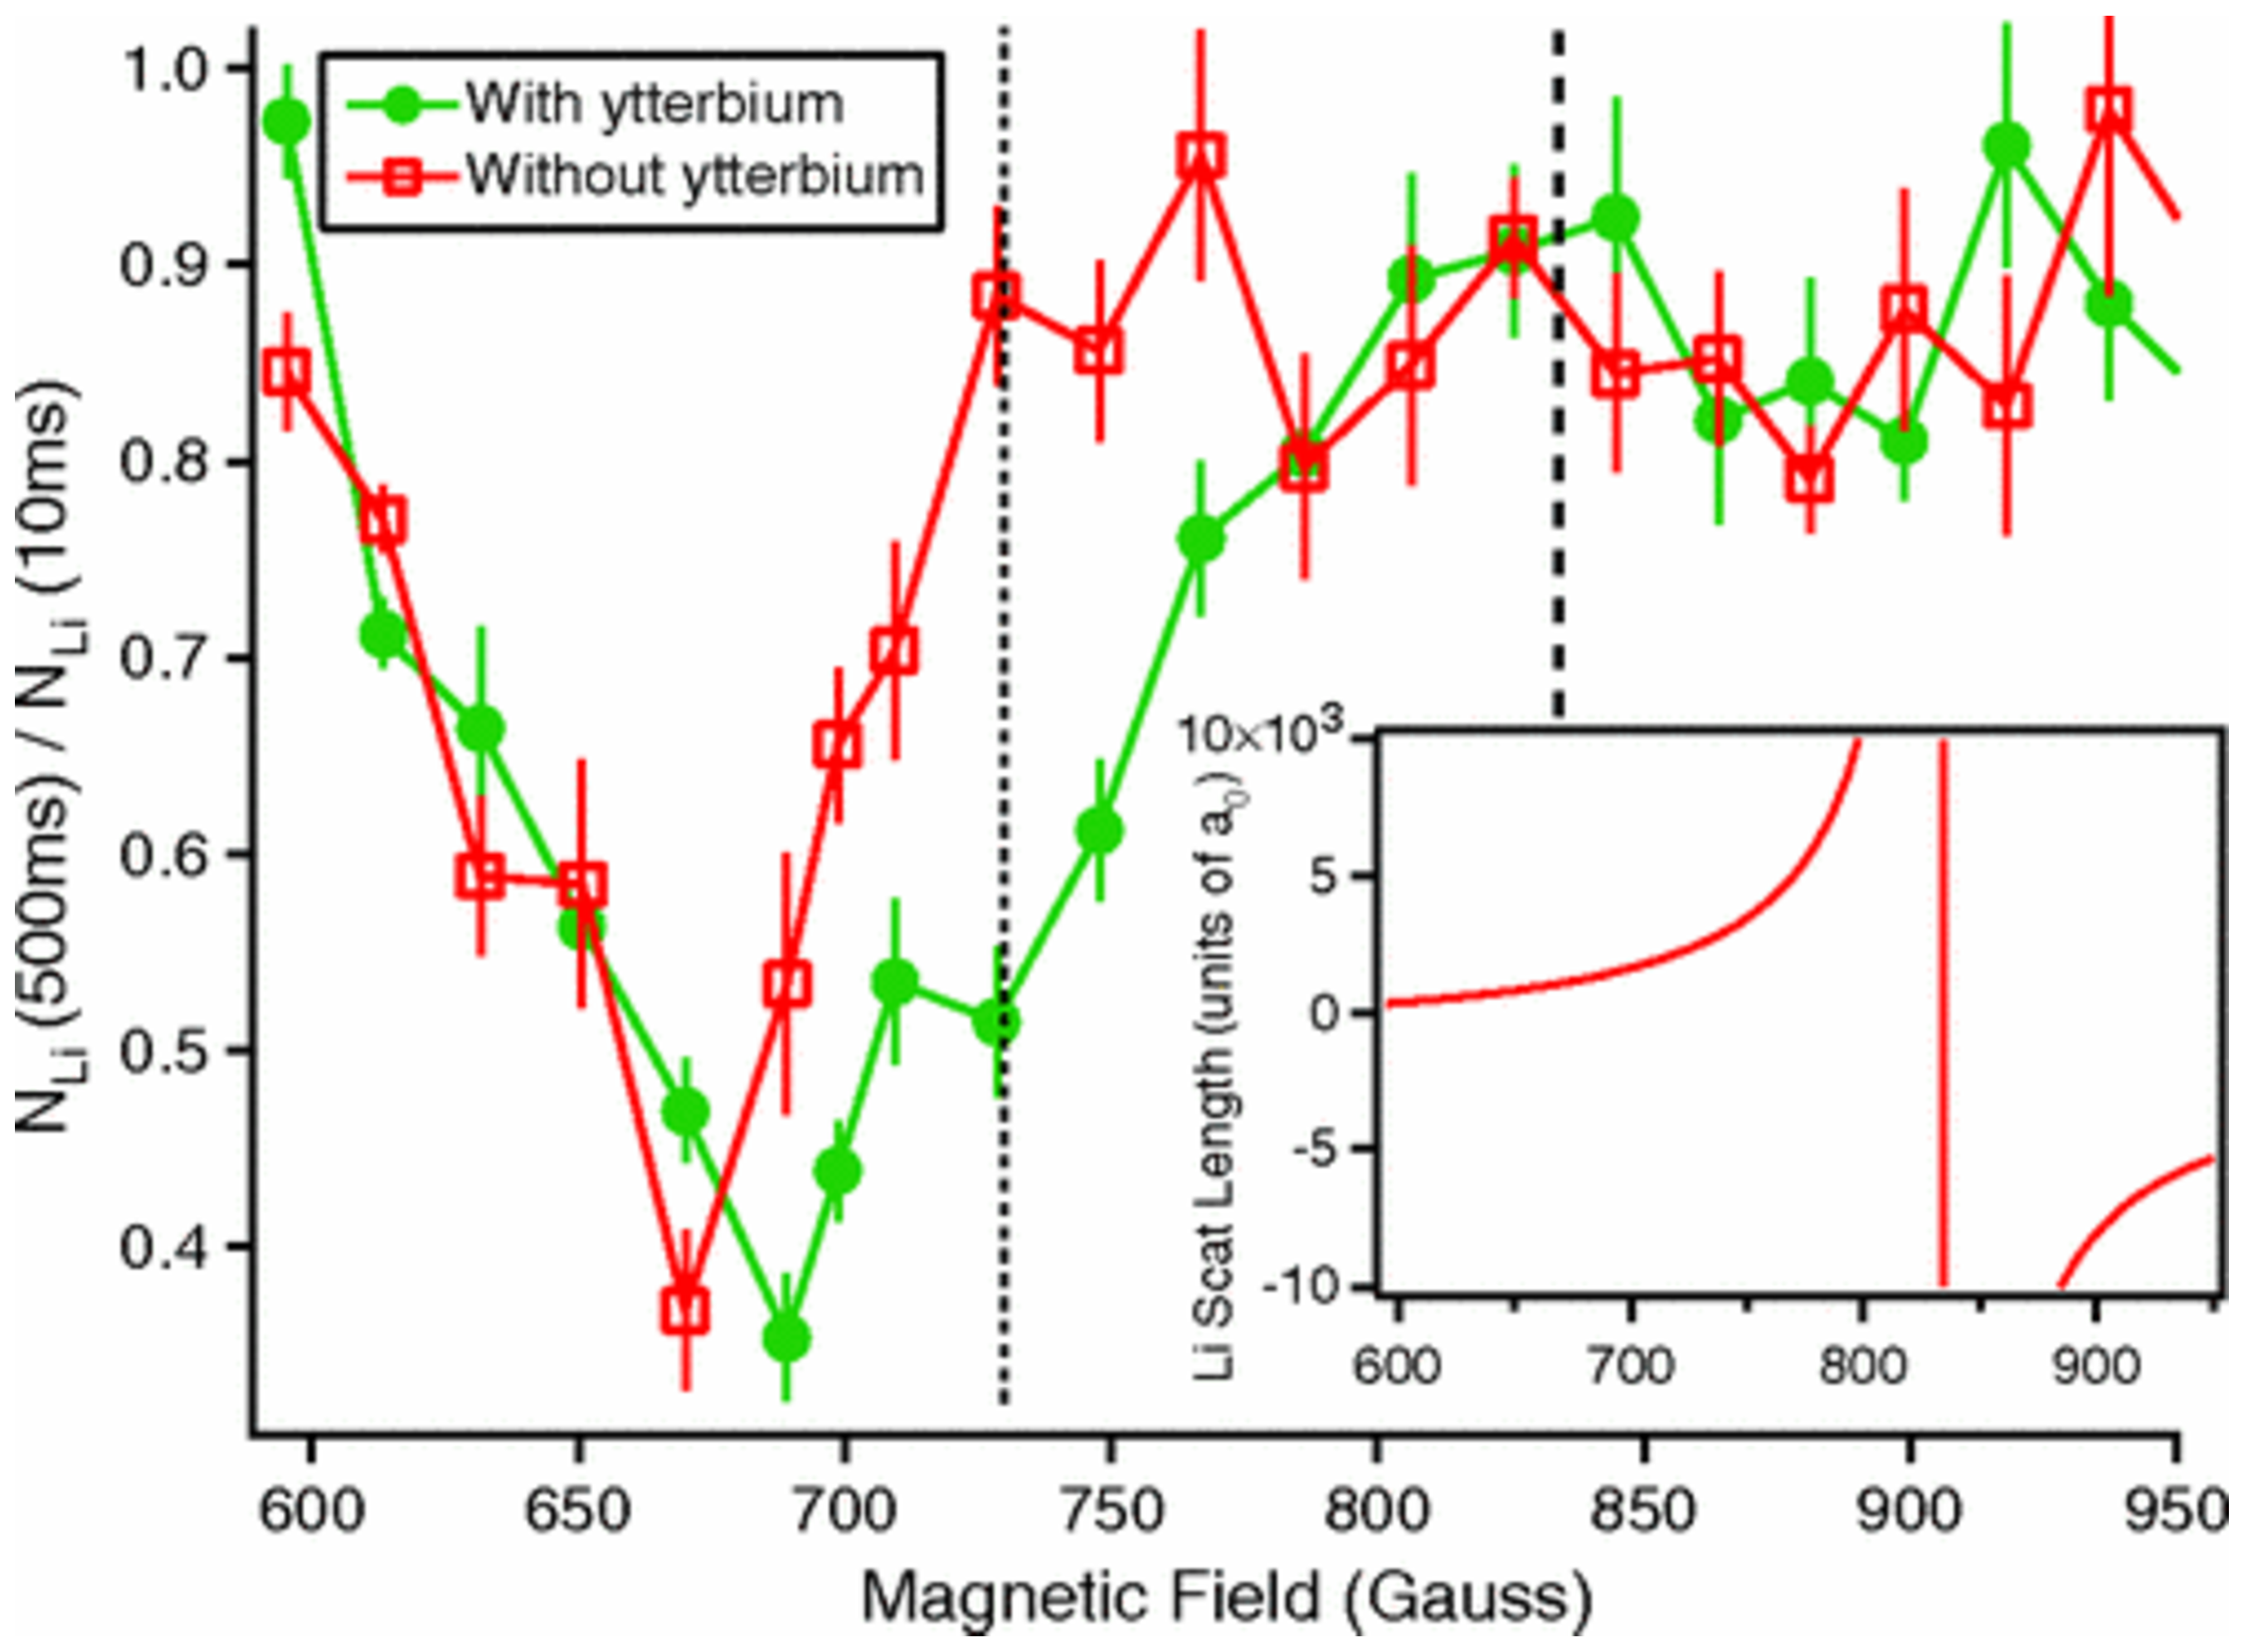
\includegraphics[width=70mm,height=50mm]{eps/imp-bcs-expe.eps}
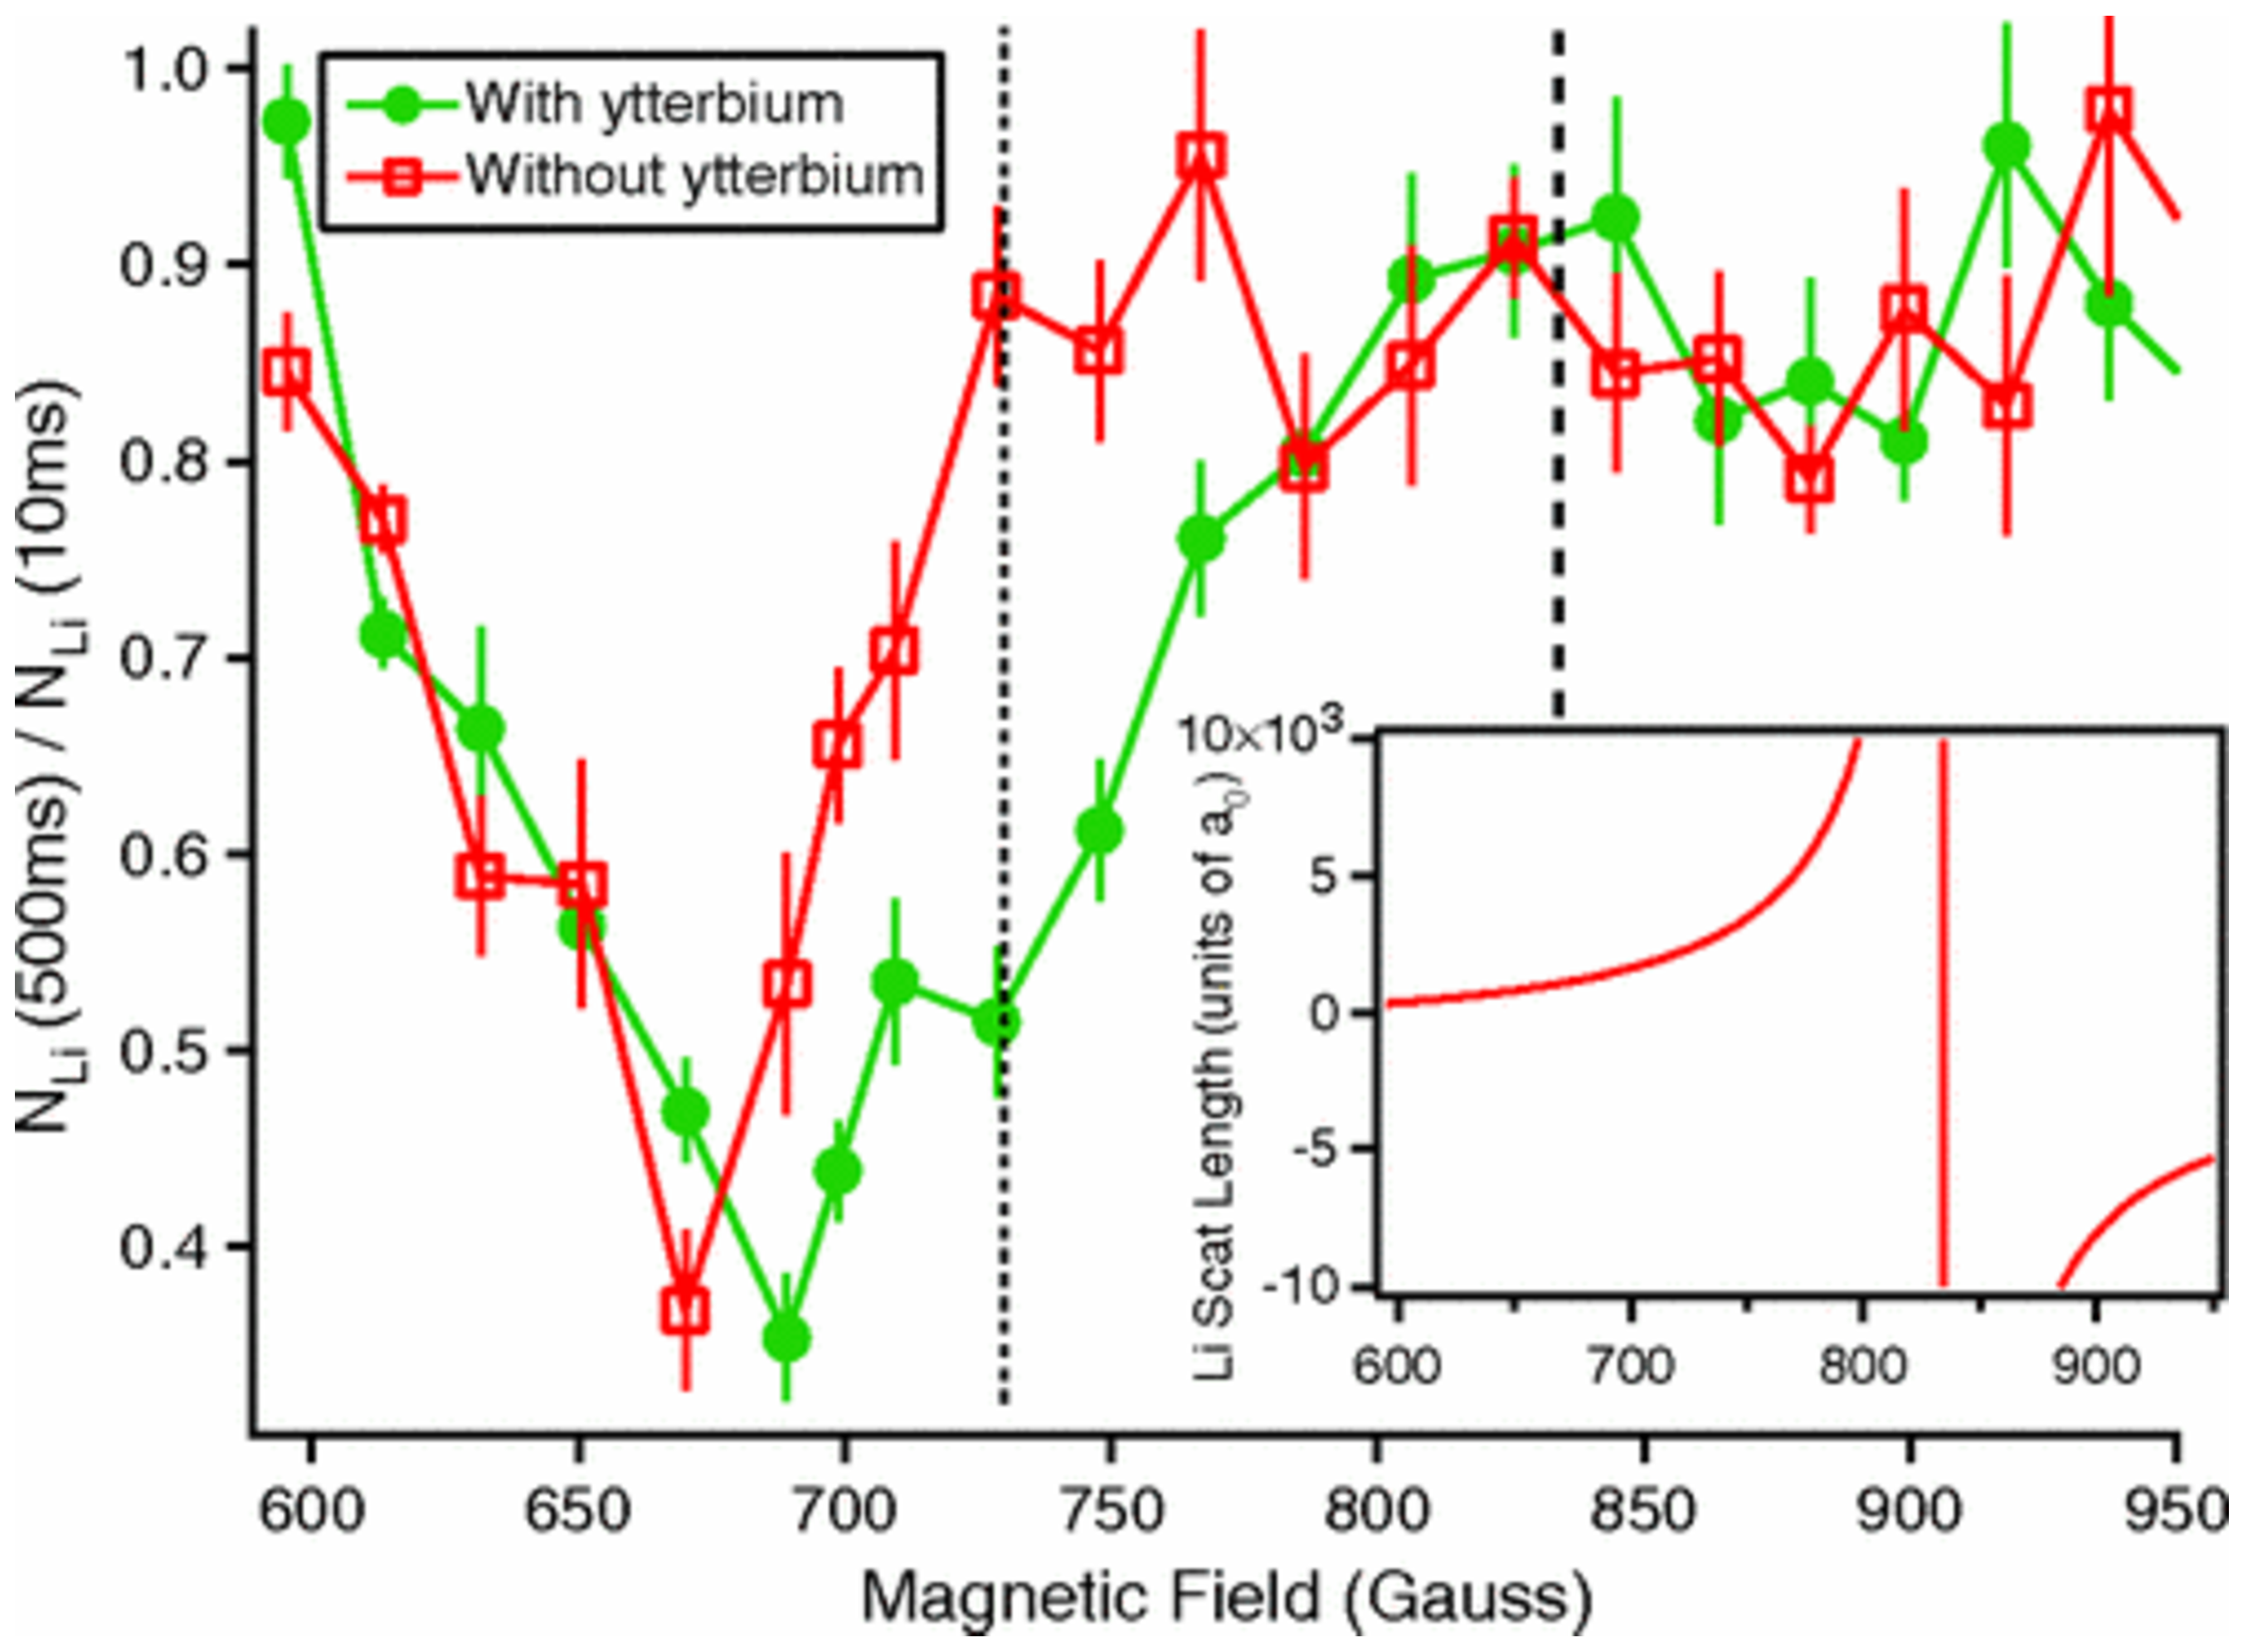
\includegraphics[width=70mm]{eps/imp-bcs-expe.eps}
\caption{$\Lisix$ フェルミ原子気体中に ${}^{174}\mathrm{Yb}$ を不純物として導入した際の $\Lisix$ 原子損失を測定した実験(緑線)\cite{kharamov2012}。赤線は ${}^{174}\mathrm{Yb}$ がない場合の結果。縦軸には $500\ \mathrm{ms}$ 後の $\mathrm{Li}$ 粒子数 $N_{\mathrm{Li}}(500\ \mathrm{ms})$ を $10\ \mathrm{ms}$ 時の $\mathrm{Li}$ 粒子数 $N_{\mathrm{Li}}(10\ \mathrm{ms})$ で規格化したもの。横軸はフェッシュバッハ磁場である。インセットは、$\Lisix$ の $s$ 波散乱長の磁場依存性。太い破線は${}^{6}\mathrm{Li}$ のフェッシュバッハ共鳴磁場 ($834\ \mathrm{G}$)を表している。系の温度は $T_{\text{Li}}=T_{\text{Yb}}=2\ \mu \mathrm{K}$ であり、$\Lisix$ のフェルミ温度を $T_{\text{F}}$、$\text{Yb}$ の BEC 温度を $T_{\text{BEC}}$ とすると、$T_{\text{Li}}/T_{\text{F}} \simeq 0.4$, $T_{\text{Yb}}/T_{\text{BEC}}\simeq 2.5$ 程度の温度まで冷却されている。}
\label{fig:imp-mixture}
\end{figure}

\begin{figure}[t]
\centering
%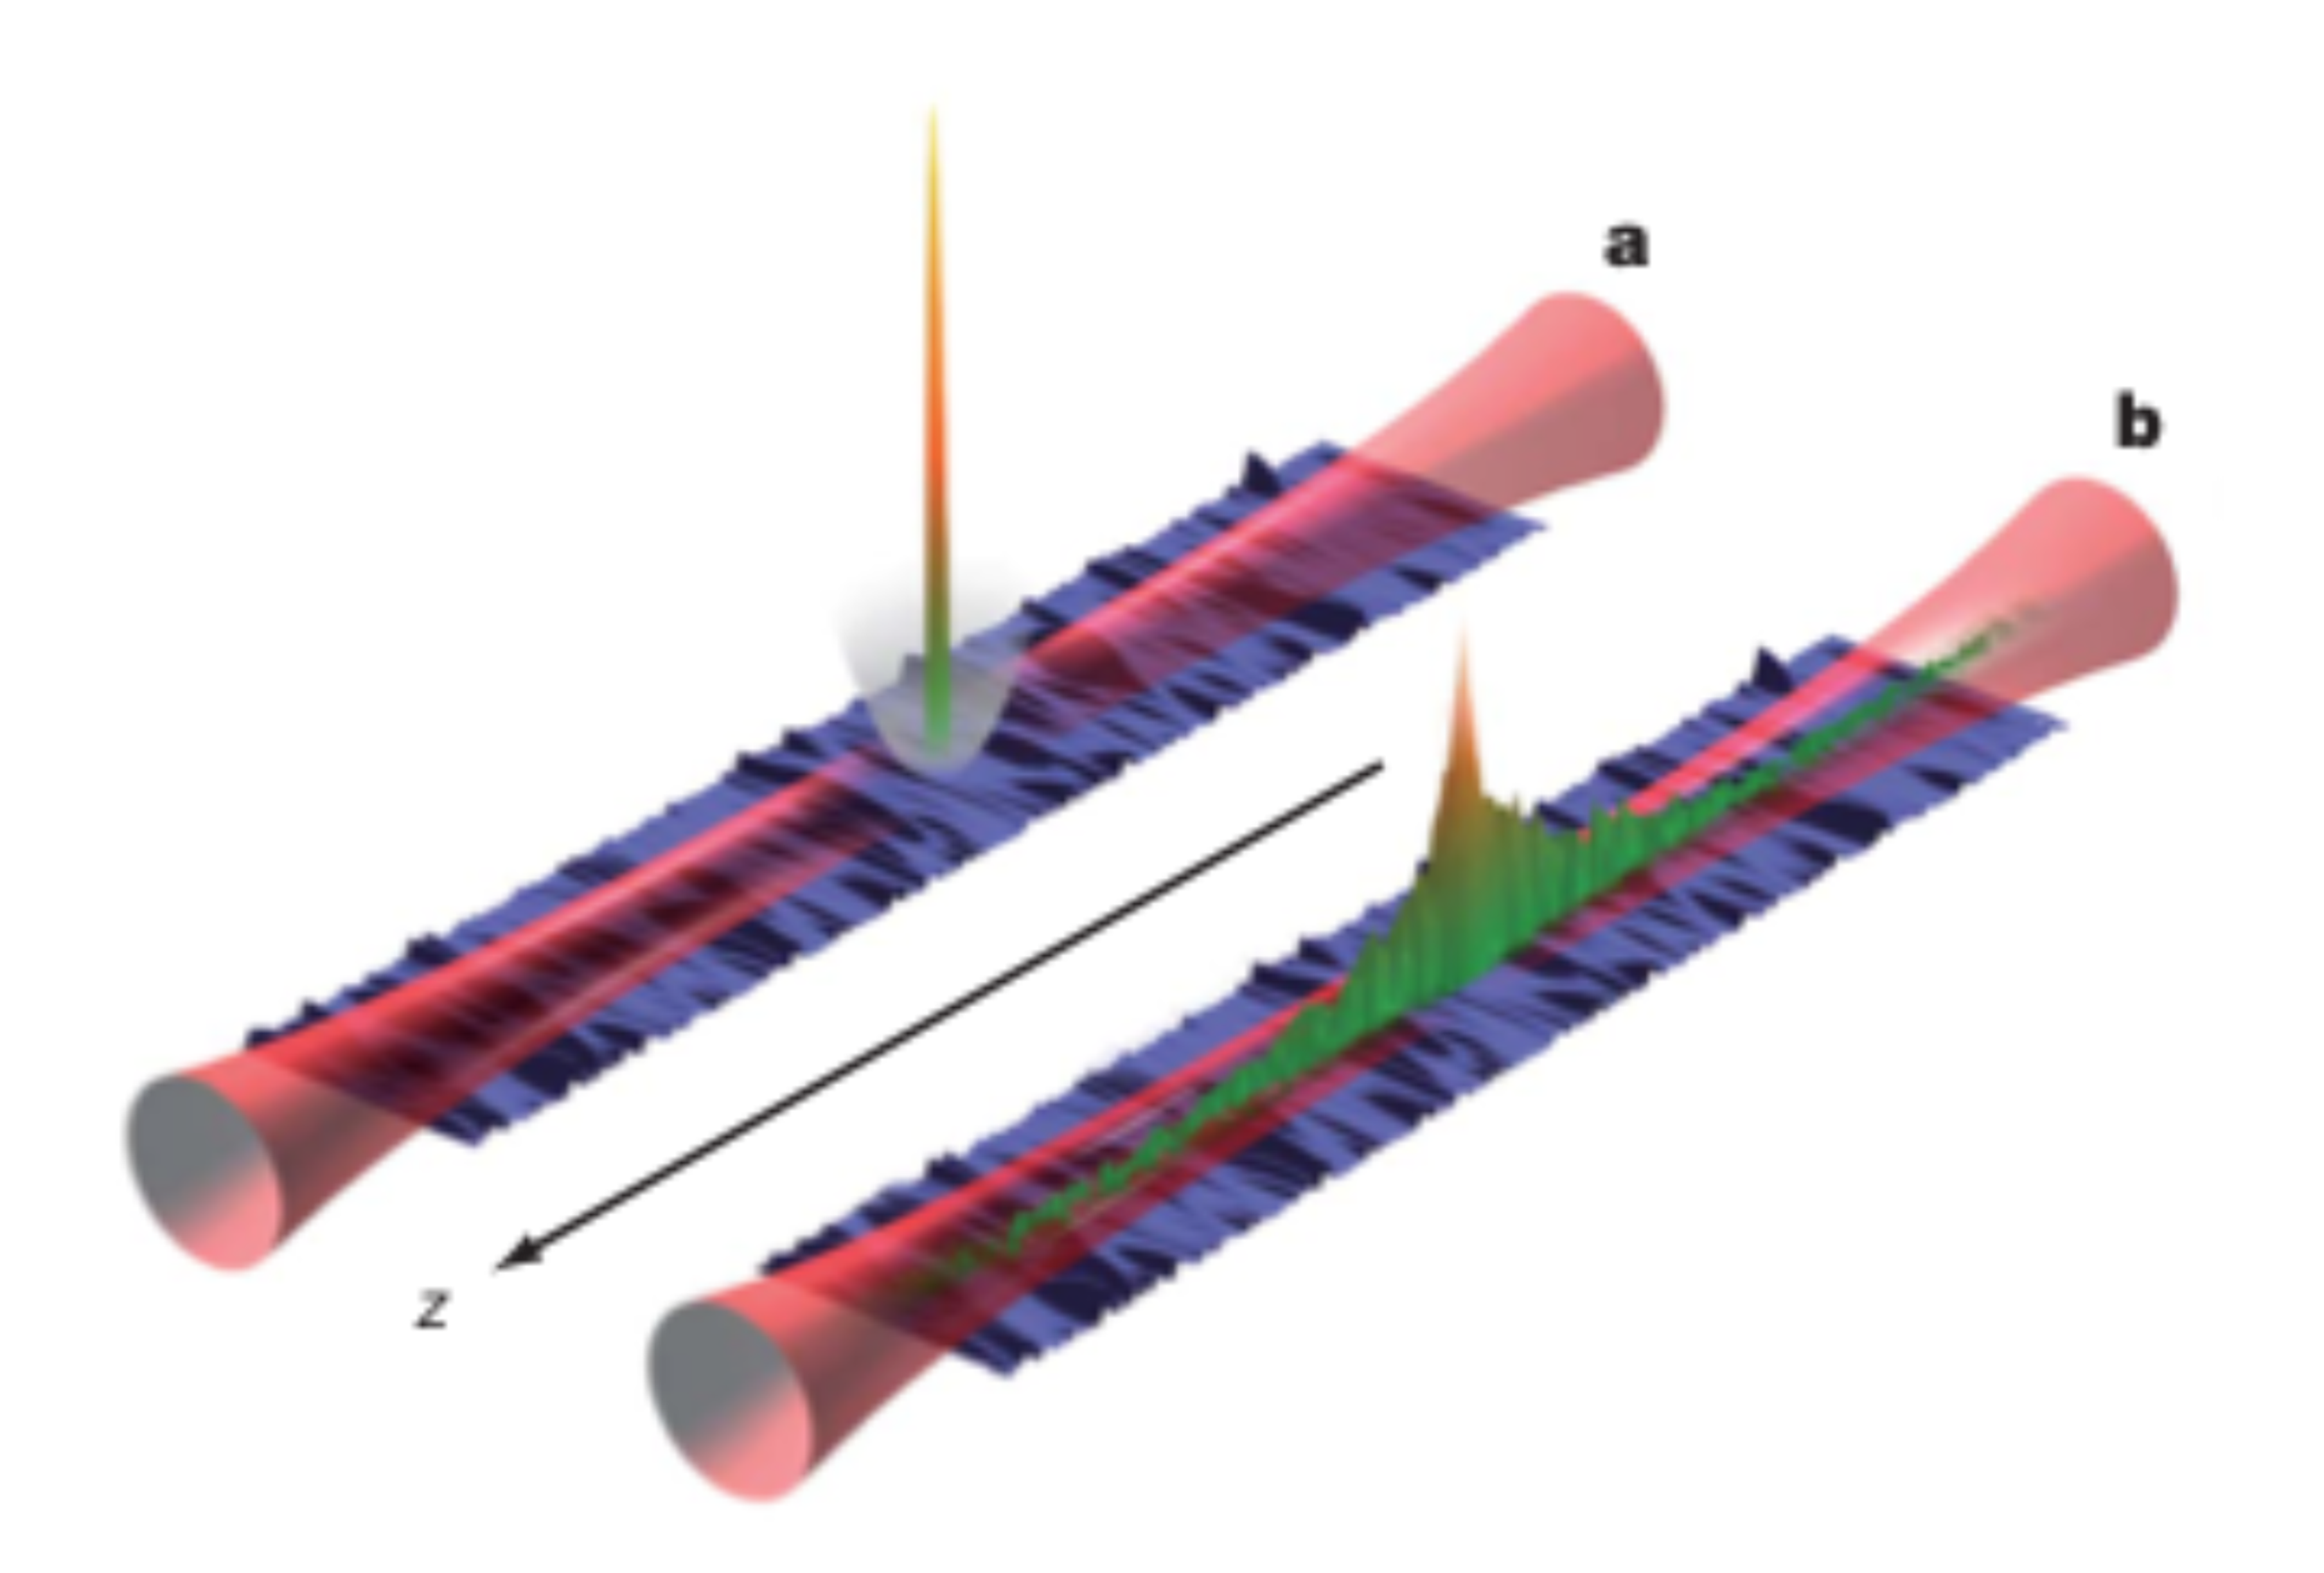
\includegraphics[width=120mm,height=70mm,draft]{eps/laser-anderson.eps}
%\vspace{30mm}  
%J. Billy, V. Josse, Z. Zuo, A. Bernard, B. Hambrecht, P. Lugan, D. Clement,\\ L. Sanchez-Palencia, P. Bouyer, and A. Aspect, Nature {\bf 453}, 891 (2008).\\
%Figure 1.
%\vspace{30mm}
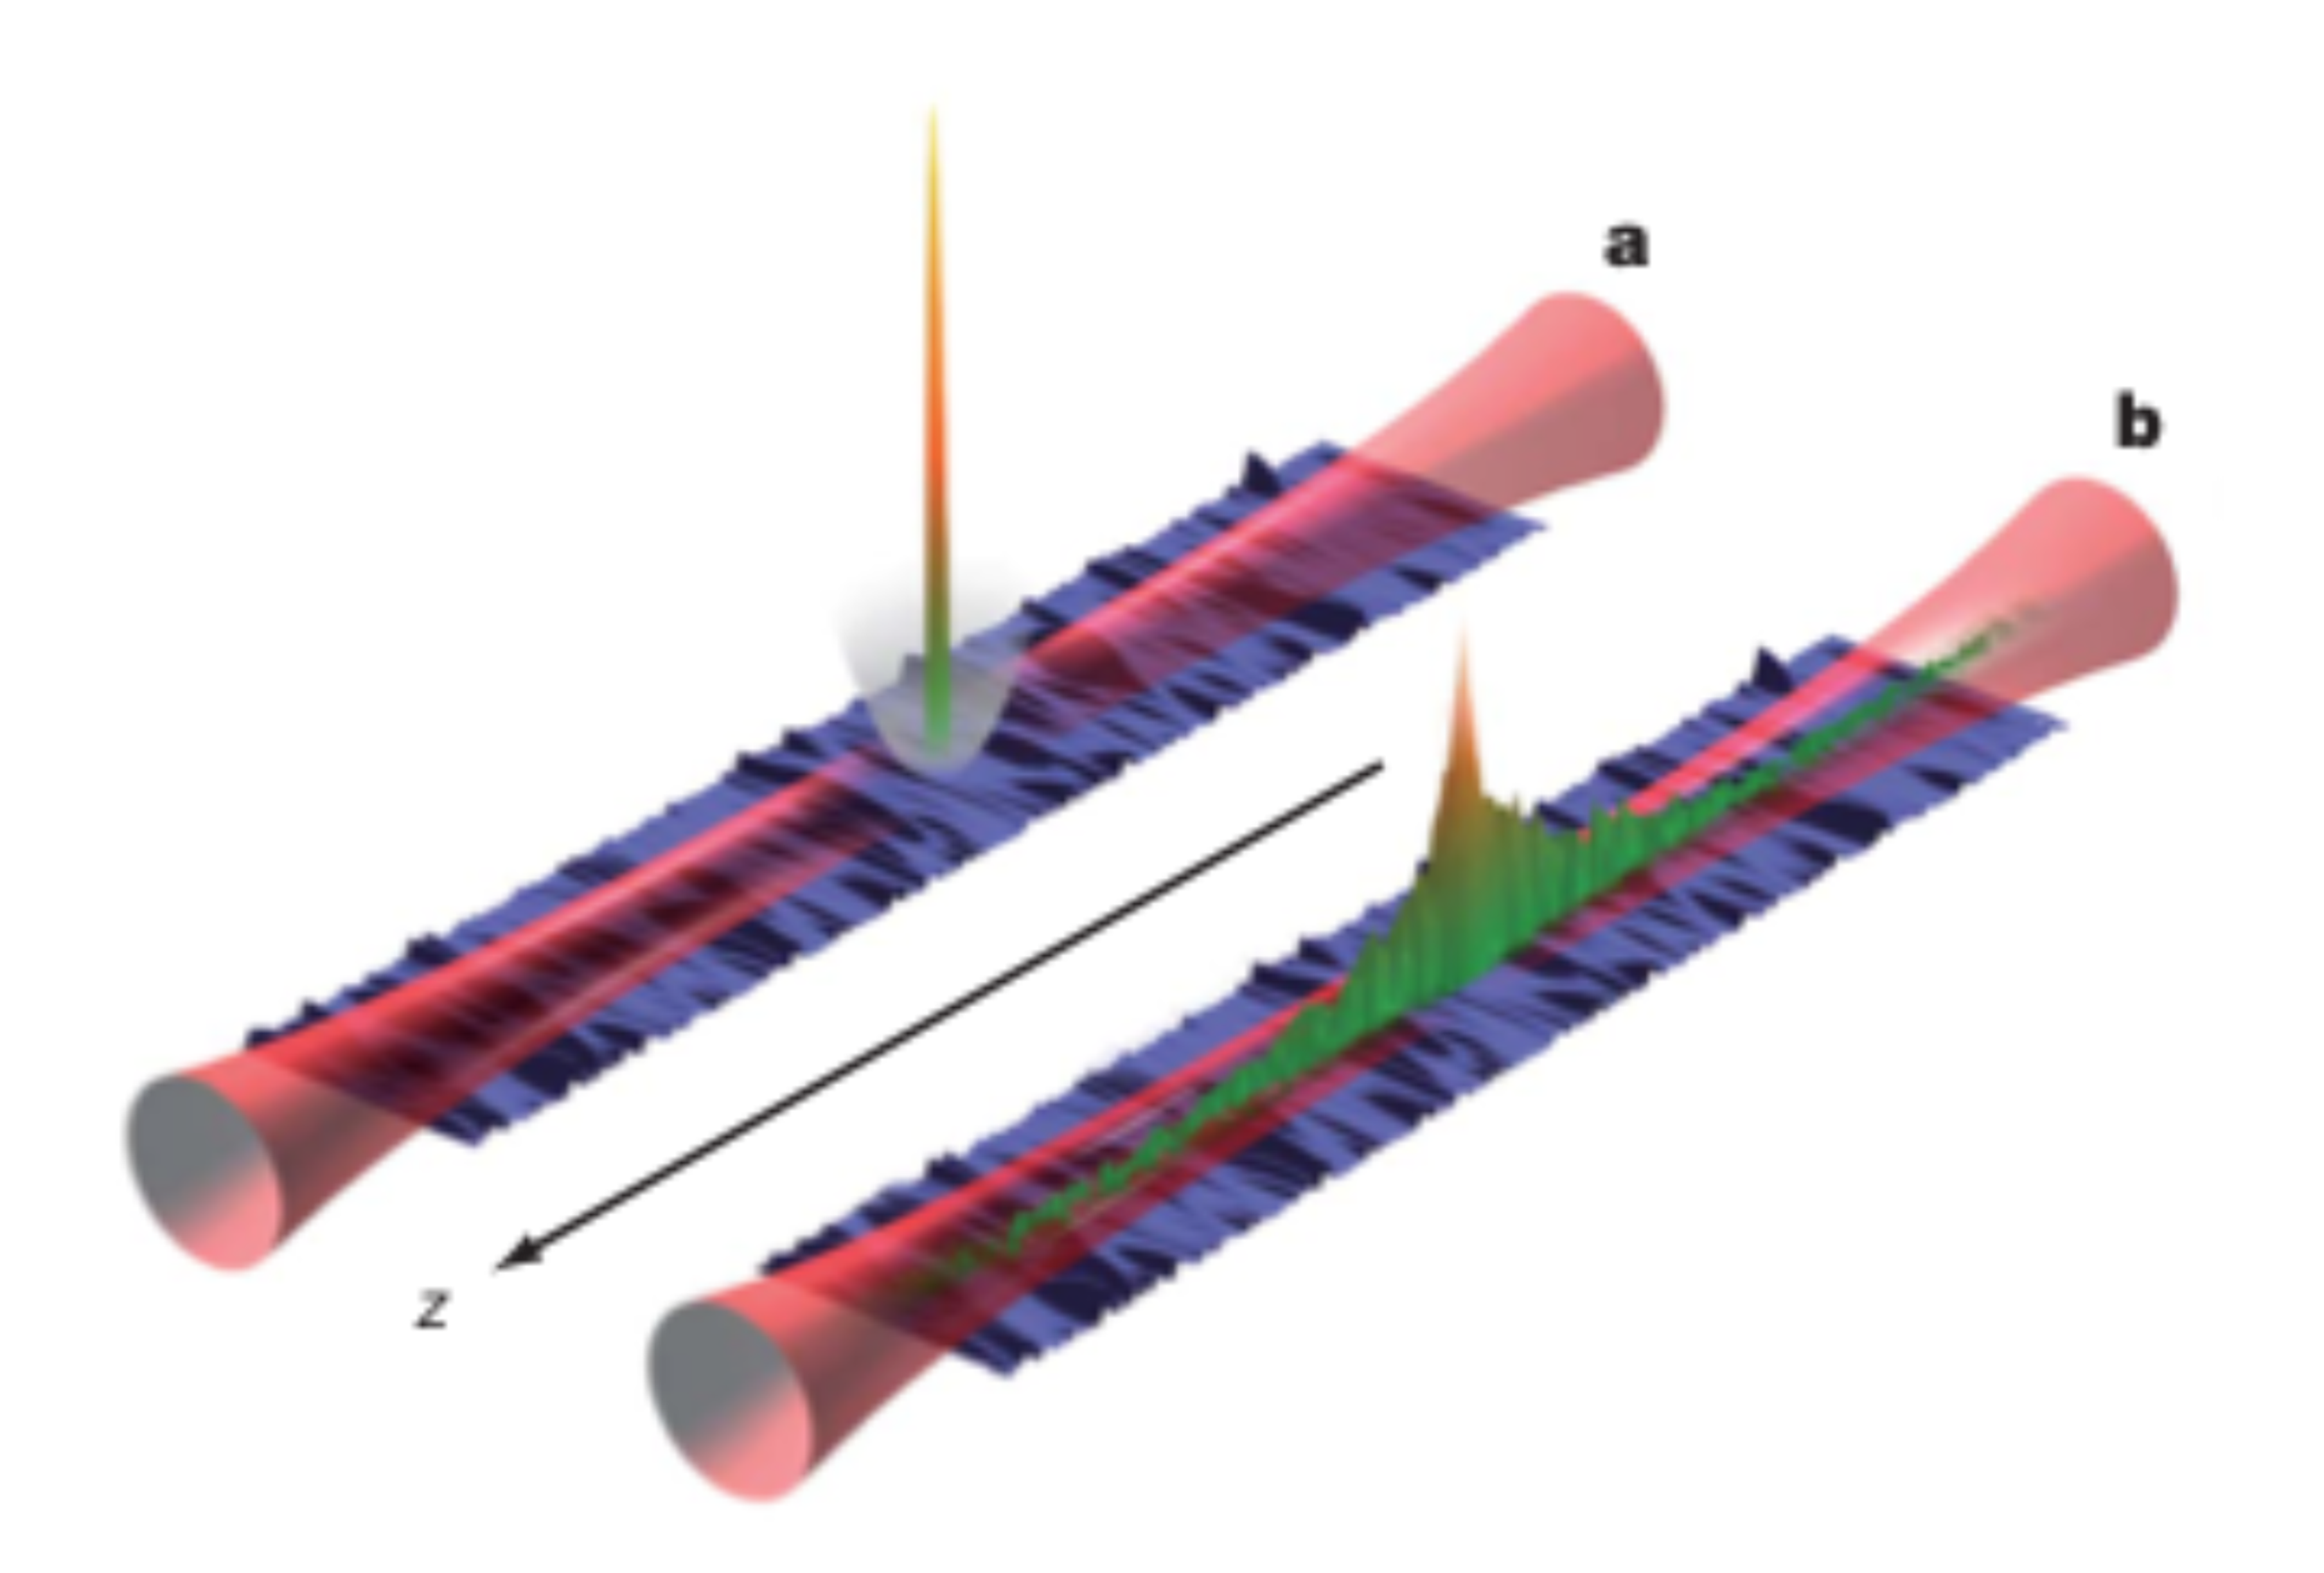
\includegraphics[width=75mm]{eps/laser-anderson.eps}
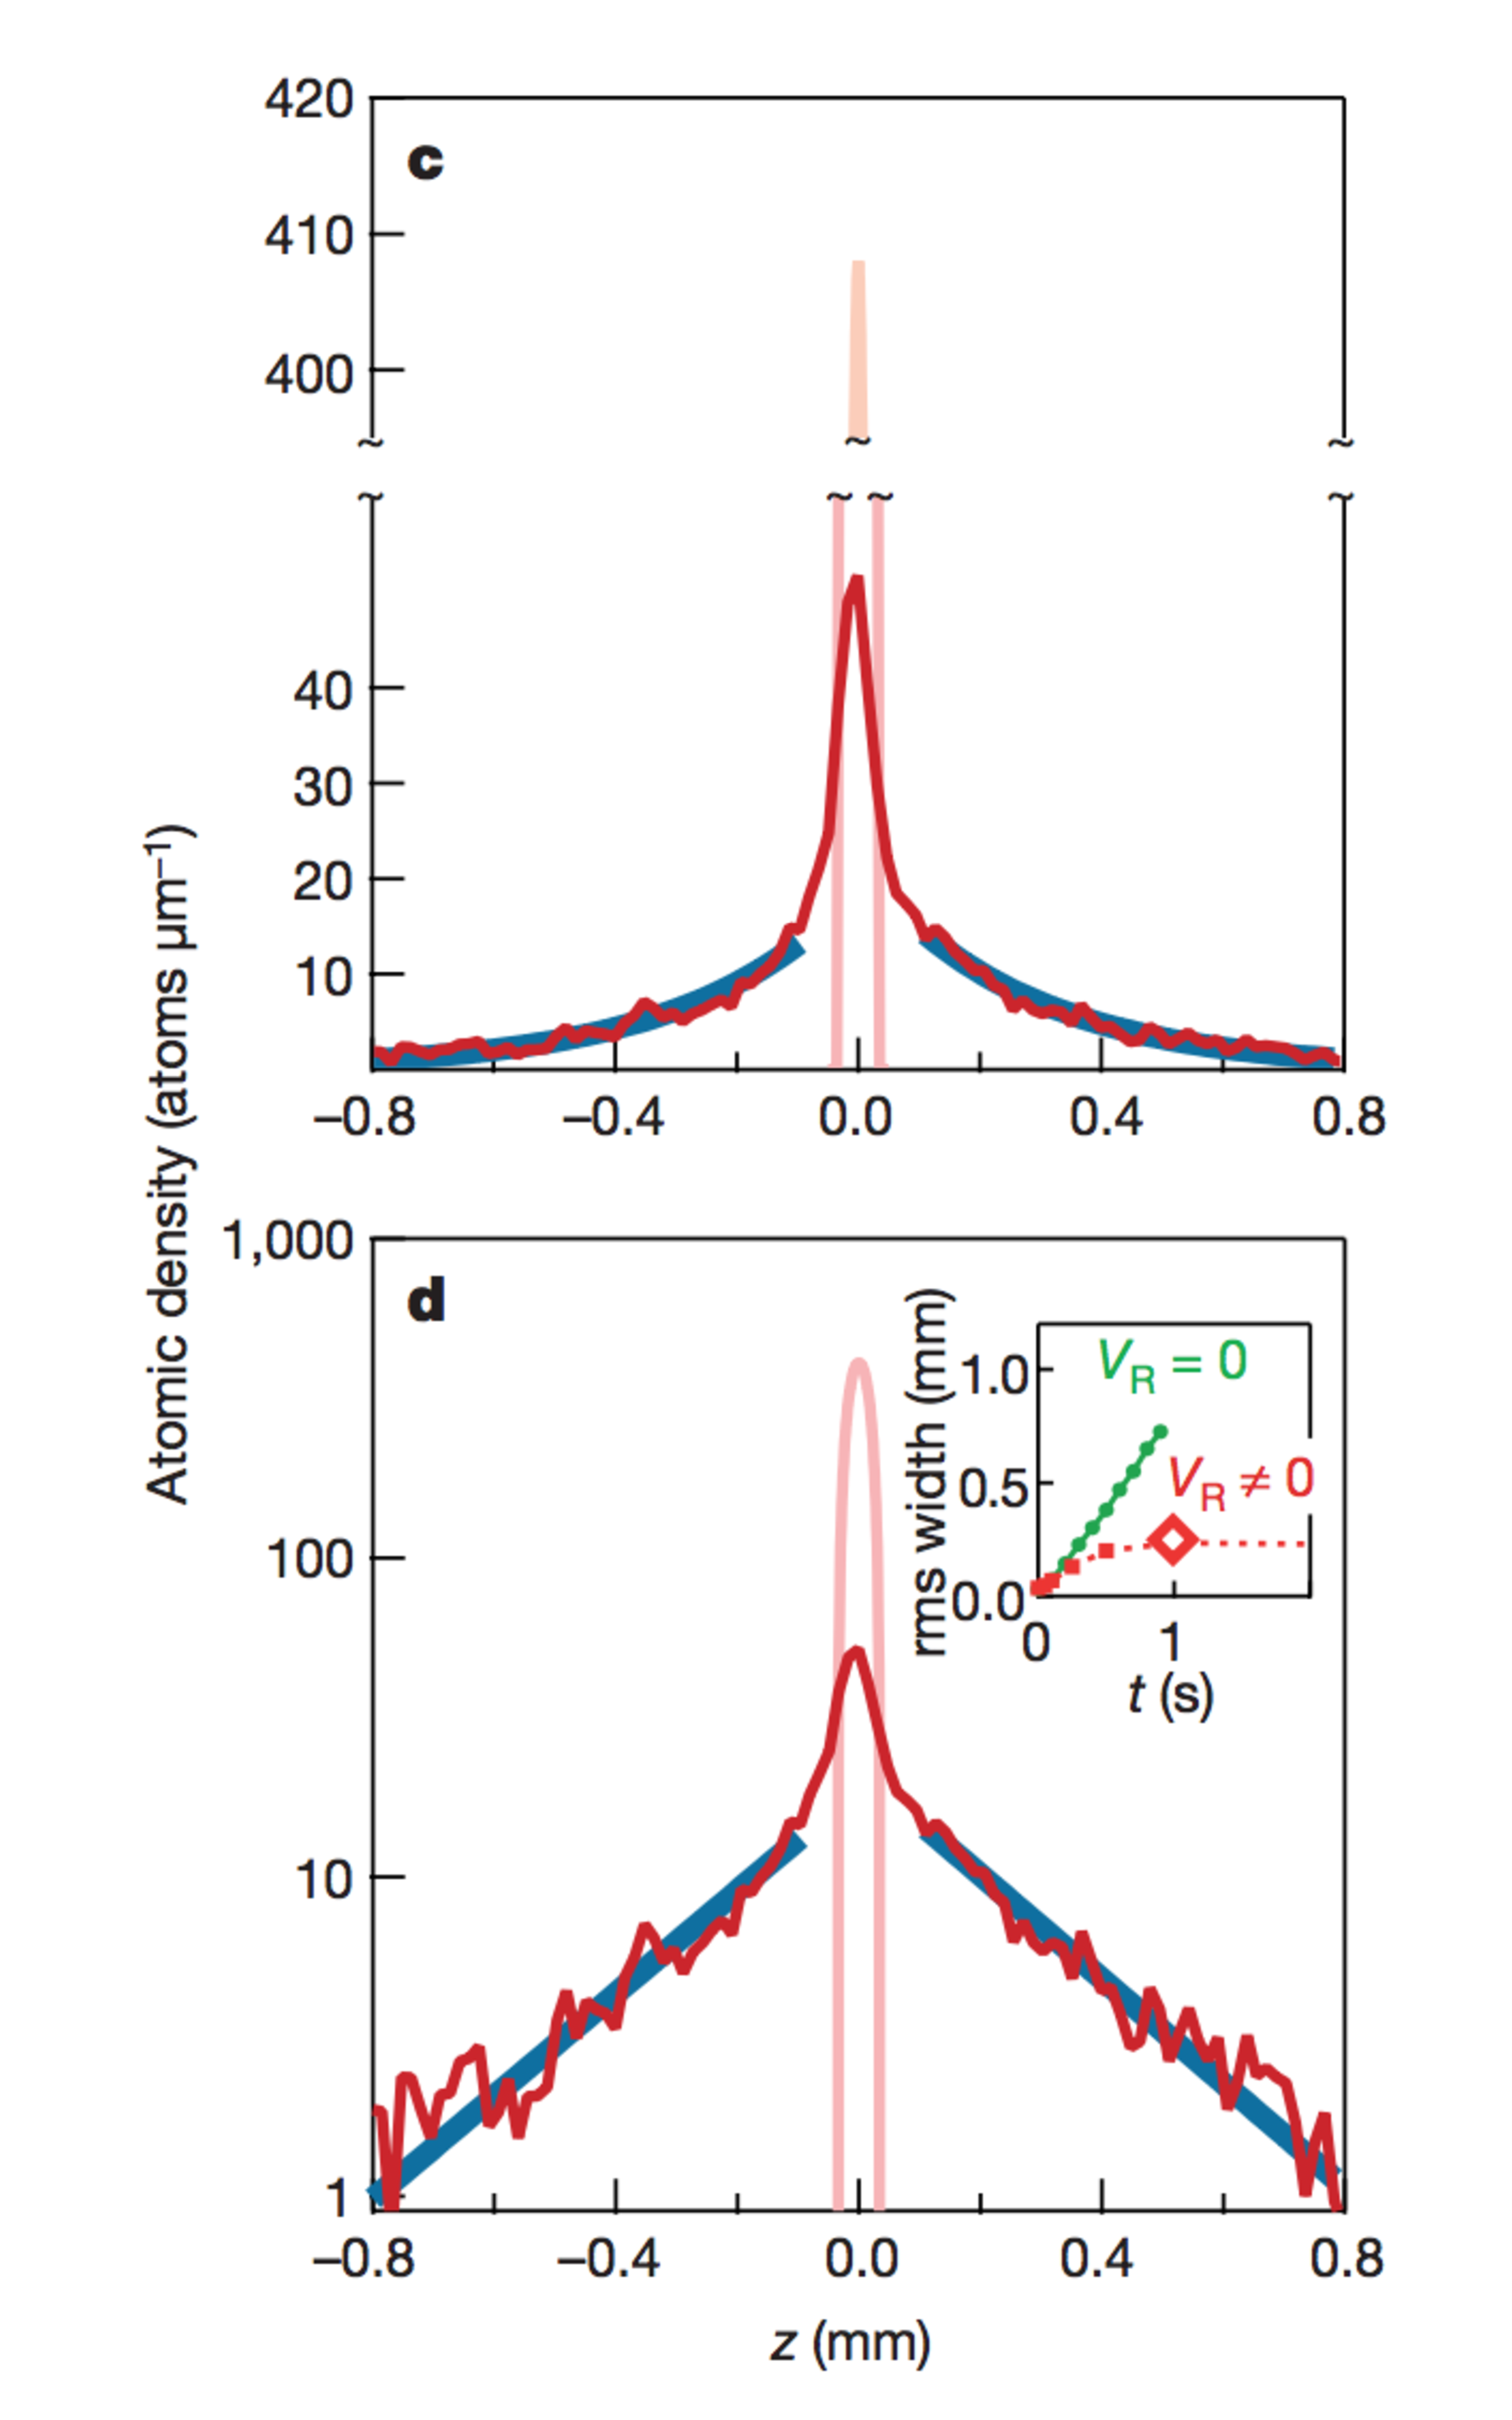
\includegraphics[width=45mm]{eps/imp-anderson-fig.eps}
\caption{一次元光学格子にランダムポテンシャルを導入した ${}^{87}\mathrm{Rb}$ ボース原子気体で観測されたアンダーソン局在 \cite{billy2008}。一次元光学格子にランダムポテンシャル $V_{\text{R}}$ を用いて乱れを導入している。(a) は初期状態であり、中央の灰色のトラップポテンシャル中には ${}^{87}\mathrm{Rb}$ の BEC (粒子数は $1.7 \times 10^4$ 程度) が形成されている。ある時刻でトラップポテンシャルをなくし、原子気体を膨張させる。(b) 解放された原子気体は次第に広がっていく。(c), (d) は解放から $1 \mathrm{s}$ 後の原子の密度分布であり、(d) のインセットは二乗平均幅の平方根 (root-mean-square width) の時間依存性を示す。ランダムポテンシャル $V_{\text{R}} =0$ の純粋系の場合には拡散していくが、$V_{\text{R}}\neq0$ の場合には、$t=0.5\ \text{s}$ 後には定常状態になっていることがわかる。(c), (d) の結果は、粒子数分布が指数的に減衰していることより、局在していることを示している。}
\label{fig:imp-localization}
\end{figure}


\s{極低温フェルミ原子気体における不純物効果の検証}

冷却フェルミ原子気体はそのままでは不純物は存在せず、背景に結晶もないガスであるため格子欠陥も存在しない。ここでは、そのような“クリーンな系”に対し、不純物の効果をどのように実験的に系に加えるかについて説明する。特にここでは原子ガス混合とレーザースペックルを用いた方法を説明する。


原子ガス混合 \cite{kharamov2012,konishi2016,hansen2011,kharamov2013,kharamov2014,hara2014} とは、$\Lisix$ といった軽い原子からなる気体に ${}^{174}\mathrm{Yb}$ などの重い原子を混合し、重い原子を静的な不純物として考えるものである。図~\ref{fig:imp-mixture} は、ボソンである ${}^{174}\mathrm{Yb}$ をフェッシュバッハ共鳴点付近の ${}^{6}\mathrm{Li}$ フェルミ原子気体に混合した実験であり、混合した状態でもユニタリー極限($B=834\ \mathrm{G}$)において、$100\ \mathrm{ms}$ の長い寿命を持った分子が観測されている \cite{kharamov2012}。原子ガス混合を用いて BCS-BEC クロスオーバー領域での不純物効果を直接観測した実験は未だ行われていないが、不純物効果を調べる道具として有望な方法の 1 つである。


冷却原子気体に不純物散乱効果を導入するもう一つの方法は、レーザースペックル等により、不規則な光ポテンシャルを導入するものである。図 \ref{fig:imp-localization} は、1 次元系においてこの方法で導入されたランダムなポテンシャルによりアンダーソン局在 \cite{andersonlocal1958} を観測した実験の結果である \cite{billy2008}。この方法による“乱れ”の導入は高次元系にも拡張され、二次元系\cite{robert2010}、三次元系\cite{Kondov2011,Jendrzejewski2011} などでも研究されている。


\s{本論文の目的と構成}

本論文の目的は、極低温フェルミ原子気体における非磁性不純物効果を BCS-BEC クロスオーバー領域で研究し、非磁性不純物が対形成に与える影響を明らかにすることである。

上記の研究を行うには、フェルミ原子間相互作用による原子同士の散乱と非磁性不純物による散乱という 2 種類の散乱効果を考慮する必要があるが、本研究ではそれぞれの散乱を次のように扱う。

まず非磁性不純物は静的な場合を考え、不純物のランダムな空間分布に対しては分布平均をとる。不純物散乱は自己無撞着 $T$ 行列近似で扱う。自己無撞着 $T$~行列近似は、金属超伝導体中の磁性不純物の周囲に Shiba 状態と呼ばれる局在励起状態が形成されることを示す際に用いられた近似であり、不純物による束縛状態を記述することができる。これに加え、冷却原子の場合には観測量のみで理論を記述するためには $T$~行列近似以上の理論を用いる必要があるため、この近似を用いる。

フェッシュバッハ共鳴による可変な引力相互作用については、先ず絶対零度の超流動状態では BCS-Leggett 理論を用いる。この理論を用い、BCS-BEC クロスオーバー領域における超流動秩序パラメータ $\del$ に対する不純物効果を明らかにする。金属超伝導におけるアンダーソンの定理とは異なり、フェルミ原子ガス超流動では非磁性不純物であっても超流動状態に影響を与えることを示す。有限温度の場合に BCS-BEC クロスオーバー全域を記述するには、超流動ゆらぎの影響を取り込む必要があるので、$T$ 行列近似を用いる。本研究では特に超流動転移温度 $\tc$ に対する不純物効果に着目し、ユニタリ極限 $\left(\askfi=0\right)$ において不純物散乱が $\tc$ をどう抑制するか、またこの領域に表れる擬ギャップ現象が不純物の存在によりどう影響を受けるか研究する。

本論文の構成は以下通りである。第 2 章では、全系のハミルトニアンを提示する。絶対零度における BCS-Leggett 理論と、超流動転移温度以上の場合に対する $T$ 行列理論を非磁性不純物効果が存在する場合にどう拡張するか説明する。第 3 章では、数値計算結果とその考察を示す。まず絶対零度における超流動秩序パラメータ $\del$ を通して非磁性不純物効果を明らかにする。次に、ユニタリー極限 $\left(\askfi=0\right)$ における超流動転移温度 $\tc$ に対する不純物効果の計算結果を示す。第 4 章では、本論文のまとめと今後の課題について述べる。

